%%%%%%%%------------------------------------------------------------------------
% This program is free software: you can redistribute it and/or modify
% it under the terms of the GNU General Public License as published by
% the Free Software Foundation, either version 3 of the License, or
% (at your option) any later version.
% 
% This program is distributed in the hope that it will be useful,
% but WITHOUT ANY WARRANTY; without even the implied warranty of
% MERCHANTABILITY or FITNESS FOR A PARTICULAR PURPOSE.  See the
% GNU General Public License for more details.
% 
% You should have received a copy of the GNU General Public License
% along with this program.  If not, see <http://www.gnu.org/licenses/>.

%%%%%%%%------------------------------------------------------------------------
%%%% 导言区 
%% 文档类型为article
\documentclass[a4paper, 11pt]{book}
%1m = 39.4 inch
%大18开 (18.5cm * 23cm)
%\usepackage[left=3.25cm, right=3.25cm, top=2.3cm,bottom=1.4cm]{geometry}
\usepackage{geometry}
\geometry{left=3.75cm,right=3.25cm,top=3cm,bottom=2.5cm}

%% en_preamble包含基本的宏包配置
%%%%%%%%------------------------------------------------------------------------
%%%% 日常所用宏包

%%设置行间距
\usepackage{setspace}

%% 控制项目列表
\usepackage{enumerate}

%% 多栏显示
\usepackage{multicol}

%% hyperref宏包,生成可定位点击的超链接,并且会生成pdf书签
\usepackage[%
    pdfstartview=FitH,%
    CJKbookmarks=true,%
    bookmarks=true,%
    bookmarksnumbered=true,%
    bookmarksopen=true,%
    colorlinks=true,%
    citecolor=blue,%
    linkcolor=blue,%
    anchorcolor=green,%
    urlcolor=blue%
]{hyperref}

%% 控制标题
\usepackage{titlesec}

%% 控制表格样式
\usepackage{booktabs}

%% 控制目录
\usepackage{titletoc}

%% 控制字体大小
\usepackage{type1cm}

%% 首行缩进,用\noindent取消某段缩进
\usepackage{indentfirst}

%% 支持彩色文本、底色、文本框等
\usepackage{color,xcolor}

%% AMS LaTeX宏包
\usepackage{amsmath}

%% 一些特殊符号
% \usepackage{bbding}

%% 支持引用
% \usepackage{cite}

%% LaTeX一些特殊符号宏包
% \usepackage{latexsym}

%% 数学公式中的黑斜体
% \usepackage{bm}

%% 调整公式字体大小:\mathsmaller, \mathlarger
% \usepackage{relsize}

%% 生成索引
% \makeindex

%%%% 基本插图方法
%% 图形宏包
\usepackage{graphicx}
\usepackage{float}
%% 如果插入的图片没有指定扩展名,那么依次搜索下面的扩展名所对应的文件
\DeclareGraphicsExtensions{.pdf,.eps,.png,.jpg}
%% 让 latex 从 .bb 中读取 Bounding Box 信息
%\DeclareGraphicsRule{.jpg}{eps}{.bb}{}
%\DeclareGraphicsRule{.png}{eps}{.bb}{}
%\DeclareGraphicsRule{.pdf}{eps}{.bb}{}

%% 多个图形并排,参加lnotes.pdf
%\usepackage{subfig}
\usepackage{subfigure}


\usepackage{caption}
\captionsetup{font={sf, scriptsize}, labelfont={bf}, skip=15pt}
\DeclareCaptionLabelSeparator{colon}{~~}

\usepackage[perpage,stable]{footmisc}

\usepackage{longtable}
% \begin{figure}[htbp]               %% 控制插图位置
%   \setlength{\abovecaptionskip}{0pt}
%   \setlength{\belowcaptionskip}{10pt}
                                     %% 控制图形和上下文的距离
%   \centering                       %% 使图形居中显示
%   \includegraphics[width=0.8\textwidth]{CTeXLive2008.jpg}
                                     %% 控制图形显示宽度为0.8\textwidth
%   \caption{CTeXLive2008安装过程} \label{fig:CTeXLive2008}
                                     %% 图形题目和交叉引用标签
% \end{figure}
%%%% 基本插图方法结束

%%%% pgf/tikz绘图宏包设置
\usepackage{pgf,tikz}
\usetikzlibrary{shapes,automata,snakes,backgrounds,arrows}
\usetikzlibrary{mindmap, trees,  calendar}
\usetikzlibrary{positioning}
\usepackage{pgf-umlsd}
%% 可以直接在latex文档中使用graphviz/dot语言,
%% 也可以用dot2tex工具将dot文件转换成tex文件再include进来
%% \usepackage[shell,pgf,outputdir={docgraphs/}]{dot2texi}
%%%% pgf/tikz设置结束


%%%% fancyhdr设置页眉页脚
%% 页眉页脚宏包
\usepackage{fancyhdr}

%% 页眉页脚风格
\pagestyle{fancy}

%%这两行代码是修改\leftmark和\rightmark的经典模式
\renewcommand{\chaptermark}[1]{\markboth{{\hei {第\thechapter{}章}}\hspace 1  #1}{}}
\renewcommand{\sectionmark}[1]{\markright{\thesection{} #1}}

%% 清空当前页眉页脚的默认设置
\fancyhf{}

%\fancyhead[L]{\scriptsize \fangsong \ascii{ZTE}中兴}
%\fancyhead[R]{\scriptsize \fangsong 内部公开}

%\fancyhead[CE]{\scriptsize \fangsong \leftmark}
%\fancyhead[CO]{\scriptsize \fangsong \rightmark}

%\fancyfoot[RO, LE]{\scriptsize \thepage}
%\fancyfoot[C]{\scriptsize \fangsong 本文中的所有信息均为中兴通讯股份有限公司内部信息,不得向外传播}

\renewcommand{\headrulewidth}{0.4pt}
\renewcommand{\footrulewidth}{0.4pt}

%第{\couriernew\thechapter{}}章
%%下面开始修改页眉和页脚
\fancyhead[RE]{\fangsong \leftmark}
\fancyhead[LO]{\fangsong \rightmark}
\fancyhead[RO, LE]{\small \thepage}
\fancypagestyle{plain}{%
  \fancyhead{} % get rid of headers
  \renewcommand{\headrulewidth}{0pt} % and the line.
}

%%定义空白页面
\makeatletter
\def\cleardoublepage{\clearpage\if@twoside \ifodd\c@page\else
  \hbox{}
  \vspace*{\fill}
  \begin{center}
   {\sffamily\large This page is intentionally left blank.}
   \end{center}
   \vspace{\fill}
   \thispagestyle{empty}
   \newpage
   \if@twocolumn\hbox{}\newpage\fi\fi\fi}
\makeatother

%% 有时会出现\headheight too small的warning
\setlength{\headheight}{15pt}
%%%% fancyhdr设置结束

%%设置行间距离
\usepackage{framed}  
%%%% listings宏包设置结束

%%%% 附录设置
\usepackage[title,titletoc,header]{appendix}
%%%% 附录设置结束

%%%% 日常宏包设置结束
%%%%%%%%------------------------------------------------------------------------

%%%%%%%%------------------------------------------------------------------------
%%%% 英文字体设置结束
%% 这里可以加入自己的英文字体设置
%%%%%%%%------------------------------------------------------------------------

%%%%%%%%------------------------------------------------------------------------
%%%% 设置常用字体字号,与MS Word相对应

%% 一号, 1.4倍行距
\newcommand{\yihao}{\fontsize{26pt}{36pt}\selectfont}
%% 二号, 1.25倍行距
\newcommand{\erhao}{\fontsize{22pt}{28pt}\selectfont}
%% 小二, 单倍行距
\newcommand{\xiaoer}{\fontsize{18pt}{18pt}\selectfont}
%% 三号, 1.5倍行距
\newcommand{\sanhao}{\fontsize{16pt}{24pt}\selectfont}
%% 小三, 1.5倍行距
\newcommand{\xiaosan}{\fontsize{15pt}{22pt}\selectfont}
%% 四号, 1.5倍行距
\newcommand{\sihao}{\fontsize{14pt}{21pt}\selectfont}
%% 半四, 1.5倍行距
\newcommand{\bansi}{\fontsize{13pt}{19.5pt}\selectfont}
%% 小四, 1.5倍行距
\newcommand{\xiaosi}{\fontsize{12pt}{18pt}\selectfont}
%% 大五, 单倍行距
\newcommand{\dawu}{\fontsize{11pt}{11pt}\selectfont}
%% 五号, 单倍行距
\newcommand{\wuhao}{\fontsize{10.5pt}{10.5pt}\selectfont}
%%%%%%%%------------------------------------------------------------------------

%%%%%%%%------------------------------------------------------------------------
%%%% 一些个性设置

%% 设定页码方式,包括arabic、roman等方式
%% \pagenumbering{arabic}

%% 有时LaTeX无从断行,产生overfull的错误,这条命令降低LaTeX断行标准
%% \sloppy

%% 设定目录显示深度\tableofcontents
%% \setcounter{tocdepth}{2}
%% 设定\listoftables显示深度
%% \setcounter{lotdepth}{2}
%% 设定\listoffigures显示深度
%% \setcounter{lofdepth}{2}

%% 中文破折号,据说来自清华模板
\newcommand{\pozhehao}{\kern0.3ex\rule[0.8ex]{2em}{0.1ex}\kern0.3ex}

%% 设定itemize环境item的符号
\renewcommand{\labelitemi}{$\bullet$}

%\makeatletter
%\@addtoreset{lstlisting}{section} 
%\makeatother

\newenvironment{enum}
{
  \begin{spacing}{1.2}
  \begin{enumerate}[1.]
    \setlength{\itemsep}{0pt} 
    \setlength{\itemindent}{2em}
    %\setlength{\listparindent}{2em}
}{%
  \end{enumerate}
  \end{spacing}
}

\newcommand{\suggest}[1]{
\tikzstyle{mybox} = [draw=black, very thick,
rectangle, rounded corners, inner sep=9pt, inner ysep=20pt]
\tikzstyle{fancytitle} =[fill=white, text=black, ellipse]
\noindent
\begin{tikzpicture}
\node [mybox] (box){%
\begin{minipage}{\textwidth}
\fangsong
#1
\end{minipage}
};
\node[fancytitle, right=10pt] at (box.north west) {\emph{建议}};
% \node[fancytitle, rounded corners] at (box.east) {$\clubsuit$};
\end{tikzpicture}
}

\newcommand{\notice}[1]{
\tikzstyle{mybox} = [draw=black, very thick,
rectangle, rounded corners, inner sep=9pt, inner ysep=20pt]
\tikzstyle{fancytitle} =[fill=white, text=black]
\noindent
\begin{tikzpicture}
\node [mybox] (box){%
\begin{minipage}{\textwidth}
\fangsong
#1
\end{minipage}
};
\node[fancytitle, right=10pt] at (box.north west) {\emph{注意}};
%\node[fancytitle, rounded corners] at (box.east) {$\clubsuit$};
\end{tikzpicture}
}

\newcommand{\tip}[1]{
\tikzstyle{mybox} = [draw=black, very thick,
rectangle, rounded corners, inner sep=9pt, inner ysep=20pt]
\tikzstyle{fancytitle} =[fill=white, text=black]
\noindent
\begin{tikzpicture}
\node [mybox] (box){%
\begin{minipage}{\textwidth}
\fangsong
#1
\end{minipage}
};
\node[fancytitle, right=10pt] at (box.north west) {\emph{提示}};
%\node[fancytitle, rounded corners] at (box.east) {$\clubsuit$};
\end{tikzpicture}
}

\newcommand\refch[1]{\ascii{第\ref{ch:#1}章(\nameref{ch:#1})}}
\newcommand\refsec[1]{\ascii{\ref{sec:#1}节(\nameref{sec:#1})}}

\newcommand\eitem[1]{\item {\itshape {#1}}}
\newcommand\cpp{\ascii{C\nobreak+\nobreak+}}
\newcommand\clang{\ascii{C}}

\newcommand\quo[1]{“#1”}

\newcommand\percent[1]{\ascii{#1\%}}

\newcommand{\trans}{\emph{事务}}
\newcommand{\act}{\emph{操作}}
\newcommand{\seqact}{\emph{顺序操作}}
\newcommand{\conact}{\emph{并发操作}}
\newcommand{\atomact}{\emph{基本操作}}
\newcommand{\syncact}{\emph{同步操作}}
\newcommand{\asynact}{\emph{异步操作}}
\newcommand{\action}[1]{\emph{\ascii{\itshape\_\_#1}}}
\newcommand{\sigwait}{\action{sig\_wait}}
\newcommand{\sigsync}{\action{sig\_sync}}
\newcommand{\sigreply}{\action{sig\_reply}}
\newcommand{\timerprot}{\action{timer\_prot}}
\newcommand{\unknownevet}{\ascii{UNKNOWN\_EVENT}}
\newcommand{\transdsl}{\ascii{Transaction DSL}}
\newcommand{\oper}[1]{\ascii{Action#1}}
\newcommand{\protproc}{\ascii{prot\_procedure}}

\newcommand{\code}[1]{\ascii{\scriptsize{\texttt{#1}}}}

%\newcommand{\Email}{\begingroup \def\UrlLeft{<}\def\UrlRight{>} \urlstyle{tt}\Url}
%\def\mailto|#1|{\href{mailto:#1}{Email|#1|}}
\newcommand{\contrib}[2]{#1\quad{\small\quad\textit{#2}}\\[1ex]}
%% 设定正文字体大小
% \renewcommand{\normalsize}{\sihao}

%%%% 个性设置结束
%%%%%%%%------------------------------------------------------------------------


%%%%%%%%------------------------------------------------------------------------
%%%% bibtex设置

%% 设定参考文献显示风格

%%%% bibtex设置结束
%%%%%%%%------------------------------------------------------------------------


%% 如果不写中文的话就不需要引用xecjk_preamble里面的配置
%%%%%%%%------------------------------------------------------------------------
%%%% xeCJK相关宏包

\usepackage{xltxtra,fontspec,xunicode}

%% \CJKsetecglue{\hskip 0.15em plus 0.05em minus 0.05em}
%% slanfont: 允许斜体
%% boldfont: 允许粗体
%% CJKnormalspaces: 仅忽略汉字之间的空白,但保留中英文之间的空白。 
%% CJKchecksingle: 避免单个汉字单独占一行。
\usepackage[slantfont, boldfont]{xeCJK} 

%% 针对中文进行断行
\XeTeXlinebreaklocale "zh"             

%% 给予TeX断行一定自由度
\XeTeXlinebreakskip = 0pt plus 1pt minus 0.1pt

%%%% xeCJK设置结束                                       
%%%%%%%%------------------------------------------------------------------------

%%%%%%%%------------------------------------------------------------------------
%%%% xeCJK字体设置

%% 设置中文标点样式,支持quanjiao、banjiao、kaiming等多种方式
\punctstyle{quanjiao}                                        
                                                     
%% 设置缺省中文字体
\setCJKmainfont[BoldFont={Adobe Heiti Std}, ItalicFont={Adobe Kaiti Std}]{Adobe Song Std}   %  FZBaoSongZ04
%% 设置中文无衬线字体
\setCJKsansfont[BoldFont={Adobe Heiti Std}, ItalicFont={Adobe Kaiti Std}]{Adobe Kaiti Std}  
%% 设置等宽字体
\setCJKmonofont{Adobe Heiti Std}                            
%\setCJKmonofont{Monaco}                            

%% 英文衬线字体
\setmainfont{Lucida Bright}                                  
%% 英文等宽字体
%\setmonofont{Courier}
\setmonofont{Monaco}                             
%\setmonofont{Consolas}                              
%% 英文无衬线字体
\setsansfont{Optima}                                   

%% 定义新字体
\setCJKfamilyfont{song}{Adobe Song Std}                     
\setCJKfamilyfont{kai}{Adobe Kaiti Std}
\setCJKfamilyfont{hei}{Adobe Heiti Std}
\setCJKfamilyfont{fangsong}{Adobe Song Std}
\setCJKfamilyfont{lisu}{LiShu}
\setCJKfamilyfont{youyuan}{Adobe Kaiti Std}

%%自定义英文字体
\newfontfamily\couriernew{Lucida Grande}
\newfontfamily\optima{Optima}
\newfontfamily\lucida{Lucida Bright}

\newcommand{\ascii}[1]{{\sffamily #1}}
\newcommand{\speak}[1]{{\itshape #1}}
\renewcommand{\emph}[1]{{\hei #1}}

%% 自定义宋体
\newcommand{\song}{\CJKfamily{song}}                       
%% 自定义楷体
\newcommand{\kai}{\CJKfamily{kai}}                         
%% 自定义黑体
\newcommand{\hei}{\CJKfamily{hei}}                         
%% 自定义仿宋体
\newcommand{\fangsong}{\CJKfamily{fangsong}}               
%% 自定义隶书
\newcommand{\lisu}{\CJKfamily{lisu}}                       
%% 自定义幼圆
\newcommand{\youyuan}{\CJKfamily{youyuan}}                 

%%%% xeCJK字体设置结束
%%%%%%%%------------------------------------------------------------------------

%%%%%%%%------------------------------------------------------------------------
%%%% 一些关于中文文档的重定义

%% 数学公式定理的重定义

\newtheorem{example}{例}[section]                                   
\newtheorem{algorithm}{算法}
%% 按section编号
\newtheorem{theorem}{定理}[section]                         
\newtheorem{definition}{定义}
\newtheorem{axiom}{公理}
\newtheorem{property}{性质}
\newtheorem{proposition}{命题}
\newtheorem{lemma}{引理}
\newtheorem{corollary}{推论}
\newtheorem{condition}{条件}
\newtheorem{conclusion}{结论}
\newtheorem{assumption}{假设}

\newtheorem{principle}{原则}[section]
\newtheorem{regulation}{规则}[section]
\newtheorem{advise}{建议}[section]
\newtheorem{concept}{概念}[section]

%% 章节等名称重定义
\renewcommand{\contentsname}{目录}     
%\renewcommand{\abstractname}{摘要}
\renewcommand{\indexname}{索引}
\renewcommand{\listfigurename}{插图目录}
\renewcommand{\listtablename}{表格目录}
\renewcommand{\figurename}{图}
\renewcommand{\tablename}{表}
\renewcommand{\appendixname}{附录}
\renewcommand{\appendixpagename}{附录}
\renewcommand{\appendixtocname}{附录}
%\renewcommand\refname{参考文献} 

%%设置内容环境
\newenvironment{content}{%
  \setlength{\parskip}{0.5\baselineskip}
  \begin{spacing}{1.5}
}{%
  \end{spacing}
  \setlength{\parskip}{-0.5\baselineskip}
  \vskip -0.5\baselineskip
}

\newenvironment{story}
{
  \setlength{\parskip}{0.5\baselineskip}
  \hbox to \textwidth{\hfil\rule{\linewidth}{0.5mm}\hfil}
  \begin{spacing}{1.5}
  \fangsong
}{%
  \end{spacing}
  \hbox to \textwidth{\hfil\rule{\linewidth}{0.5mm}\hfil}
  \setlength{\parskip}{-0.5\baselineskip}
  \vskip -0.5\baselineskip
}

%% 设置chapter、section与subsection的格式
%\titleformat{\chapter}[display]{\flushright\yihao}{\thechapter{}}{1em}{\textbf}
\titleformat{\section}[block]{\flushleft\sanhao}{\optima{\thesection}}{1em}{\textbf}
\titleformat{\subsection}{\sihao}{\optima{\thesubsection}}{0.5em}{\textbf}
\titleformat{\subsubsection}{\xiaosi}{\thesubsubsection}{0.5em}{\textbf}

%\titlespacing{\chapter}{0pt}{0pt}{-\baselineskip}
\titlespacing{\section}{0pt}{0pt}{0\baselineskip}
\titlespacing{\subsection}{0pt}{0.5\baselineskip}{0\baselineskip}

%% 设置章格式
\usepackage{quotchap}

\renewcommand\chapterheadstartvskip{
   \vspace*{-5\baselineskip}
}

\renewcommand\chapterheadendvskip{
   \vspace*{0.5\baselineskip}
}

\usepackage{helvet}
\renewcommand\sectfont{\rmfamily\bfseries}

\newcommand\refig[1]{{\itshape \figurename\ascii{\ref{fig:#1}(第\pageref{fig:#1}页)}}}
\newcommand\reftbl[1]{{\itshape \tablename\ascii{\ref{tbl:#1}(第\pageref{tbl:#1}页)}}}

\renewcommand{\footnoterule}{\vspace*{3pt}%
  \hrule width 0.382\textwidth height 0.4pt \vspace*{2.6pt}}
  
%%%% 中文重定义结束
%%%%%%%%------------------------------------------------------------------------


%%%% 设置listings宏包用来粘贴源代码
%% 方便粘贴源代码,部分代码高亮功能
\usepackage{listings}
\usepackage{color}

\DeclareCaptionFont{red}{\color{red}}

%% 所要粘贴代码的编程语言
\lstloadlanguages{{[LaTeX]TeX}, {[ISO]C++}, {Java}, {Ruby}}

%% 设置listings宏包的一些全局样式
%% 参考http://hi.baidu.com/shawpinlee/blog/item/9ec431cbae28e41cbe09e6e4.html
\lstset{
numberbychapter=true,
breakatwhitespace=true,
showstringspaces=false,              %% 设定是否显示代码之间的空格符号
basicstyle=\scriptsize\ttfamily,           %% 设定字体大小\tiny, \small, \Large等等
keywordstyle=\bfseries,
commentstyle=\color{red!50!green!50!blue!50},                           
escapechar=`,                        %% 中文逃逸字符,用于中英混排
xleftmargin=1.5em,xrightmargin=0em, aboveskip=1em,
breaklines,                          %% 这条命令可以让LaTeX自动将长的代码行换行排版
extendedchars=false,                 %% 这一条命令可以解决代码跨页时,章节标题,页眉等汉字不显示的问题
frameround=fttt,
captionpos=top,
belowcaptionskip=1em
}

\lstdefinestyle{numbers}{
   numbers=left,
   numberstyle=\tiny,
   stepnumber=1,
   numbersep=1em
}

\lstdefinestyle{C++}{
   language=C++,
   texcl=true,
   prebreak=\textbackslash,
   breakindent=1em,
   keywordstyle=\bfseries, %% 关键字高亮
   morekeywords={alignas, alignof, char16_t, char32_t, constexpr, decltype, noexcept, nullptr, static_assert, thread_local, override, OVERRIDE, INTERFACE, ABSTRACT, DEFINE_ROLE, ROLE, HAS_ROLE, USE_ROLE}
   style=numbers,
   %frame=leftline,                     %% 给代码加框
   %framerule=2pt,
   %rulesep=5pt
}

\lstnewenvironment{c++}[1][]
  {\setstretch{1}
  \lstset{style=C++, #1}}
  {}

%\captionsetup[lstlisting]{textfont=red}
%{labelfont=bf, singlelinecheck=off, labelsep=space, textfont=red}

\lstdefinestyle{Java}{
   language=Java,
   texcl=true,
   prebreak=\textbackslash,
   breakindent=1em,
   keywordstyle=\bfseries, %% 关键字高亮
   morekeywords={}
   style=numbers,
   %frame=leftline,                     %% 给代码加框
   %framerule=2pt,
   %rulesep=5pt
}

\lstnewenvironment{java}[1][]
  {\setstretch{1}
  \lstset{style=Java, #1}}
  {}

\lstdefinestyle{Ruby}{
   language=Java,
   texcl=true,
   prebreak=\textbackslash,
   breakindent=1em,
   keywordstyle=\bfseries, %% 关键字高亮
   morekeywords={}
   style=numbers,
   %frame=leftline,                     %% 给代码加框
   %framerule=2pt,
   %rulesep=5pt
}

\lstnewenvironment{ruby}[1][]
  {\setstretch{1}
  \lstset{style=Ruby, #1}}
  {}

\renewcommand{\lstlistingname}{示例代码}
\renewcommand\thefigure{\thechapter-\arabic{figure}}

\newcommand\refcode[1]{{\itshape \lstlistingname\ascii{\ref{code:#1}(第\pageref{code:#1}页)}}}


\usepackage[
  placement=center,
  angle=45,
  scale=4,
  color=black!40,
  %hshift=60,
  %vshift=-5
]{background}

\backgroundsetup{contents={C++ Optimal Construction Kit}}
%\backgroundsetup{contents={\includegraphics[width=0.2\textwidth]{figures/cock.jpg}}}

\newcommand{\myclearpage}{\clearpage{\pagestyle{empty}\cleardoublepage}}

%%%% 导言区结束
%%%%%%%%------------------------------------------------------------------------

%%%%%%%%------------------------------------------------------------------------
%%%% 正文部分

\begin{document}
\frontmatter
\pagestyle{empty}

%%自定义封面
\def\titlename{C++ Programming Style}
\def\subtitle{\ascii{Guidelines, Rules, and Patterns}}
\def\authors{张钟元}
\def\orgnization{\ascii{北京邮电大学}}


\newlength{\centeroffset}
\setlength{\centeroffset}{-0.5\oddsidemargin}
\addtolength{\centeroffset}{0.5\evensidemargin}
\thispagestyle{empty}

% \begin{tikzpicture}
%   \path[mindmap,concept color=black,text=white]
%     node[concept] {\ascii{Programming}}
%     [clockwise from=0]
%     child[concept color=green!50!black] {
%       node[concept] {\ascii{XP}}
%       [clockwise from=90]
%       child { node[concept] {\ascii{Simple Design}} }
%       child { node[concept] {\ascii{TDD}} }
%       child { node[concept] {\ascii{Refactoring}} }
%       child { node[concept] {\ascii{Pair Programming}} }
%     }
%     child[concept color=blue] {
%       node[concept] {\ascii{Oriented-Object}}
%       [clockwise from=-30]
%       child { node[concept] {\ascii{C++}} }
%       child { node[concept] {\ascii{Java}} }
%     }
%     child[concept color=red]
%     { node[concept] {\ascii{Evolutionary Design}} }
%     child[concept color=orange]
%     { node[concept] {\ascii{Clean Code}} };
%  \end{tikzpicture}

%title and subtitle
\vspace*{\stretch{1}}
\noindent\hspace*{\centeroffset}\makebox[0pt][l]{\begin{minipage}{\textwidth}
\flushright
{\Huge \hei \bfseries \titlename}
\noindent\rule[-1ex]{\textwidth}{5pt}\\[2.5ex]
\hfill\emph{\subtitle}
\end{minipage}}

%author
\vspace{\stretch{2}}
\noindent\hspace*{\centeroffset}\makebox[0pt][l]{\begin{minipage}{\textwidth}
\center
{\bfseries \authors} \\[1.5ex]
{\bfseries \orgnization}
\end{minipage}}

\vspace{\stretch{1}}

\pagebreak

\myclearpage

\tableofcontents
\myclearpage

\chapter{前言} 
\label{ch:preface}

\begin{content}

\ascii{C++ Programming Style}是一份关于\ascii{C++}的代码规范,为\ascii{C++}程序员提供程序设计的参考和建议。

规范总结了我们长期在编码实践中遇到的一些宝贵经验,其中部分规则、原则和建议摘自社区软件设计大师的论文、报告、书籍和博客,并引用了一些典型的源代码。

\end{content}

\section*{约定}

\begin{content}

\begin{table}[!htb]
\resizebox{0.95\textwidth}{!} {
\begin{tabular*}{1.2\textwidth}{@{}ll@{}}
\toprule
\ascii{约定} & \ascii{说明} \\
\midrule
\ascii{原则} & \ascii{坚持遵守的指导思想} \\
\ascii{规则} & \ascii{必须遵守的约定} \\ 
\ascii{建议} & \ascii{可以考虑的约定} \\ 
\ascii{正例} & \ascii{原则、规则、建议所给出的正确例子} \\ 
\ascii{反例} & \ascii{原则、规则、建议所给出的错误例子} \\ 
\bottomrule
\end{tabular*}
}
\caption{规范约定}
\label{tbl:regulation-tbl}
\end{table}

\end{content}

\section*{宏定义}

\begin{content}

为了提高代码的表现力,规范中使用了一部分实用的宏定义。为了避免歧义,这里列出了部分较为重要的宏定义供参考和查阅。

\begin{leftbar}
\begin{c++}[caption={\ttfamily{cub/base/Default.h}}]
#ifndef GKOQWPRT_1038935_NCVBNMZHJS_8909603
#define GKOQWPRT_1038935_NCVBNMZHJS_8909603

namespace details
{
   template <typename T>
   struct DefaultValue
   {
      static T value()
      {
         return T();
      }
   };

   template <typename T>
   struct DefaultValue<T*>
   {
       static T* value()
       {
           return 0;
       }
   };

   template <typename T>
   struct DefaultValue<const T*>
   {
       static T* value()
       {
           return 0;
       }
   };

   template <>
   struct DefaultValue<void>
   {
      static void value()
      {
      }
   };
}

#define DEFAULT(type, method)  \
    virtual type method { return ::details::DefaultValue<type>::value(); }

#endif
\end{c++}
\end{leftbar}

\ascii{DEFAULT}对于定义空实现的\ascii{virtual}函数非常方便。需要注意的是,\ascii{DEFAULT}所有计算都是发生在编译时,并没有任何运行时成本。

\begin{leftbar}
\begin{c++}[caption={\ttfamily{cub/base/Keywords.h}}]
#ifndef H16274882_9153_4DB2_A2E2_F23D4CCB9381
#define H16274882_9153_4DB2_A2E2_F23D4CCB9381

#include <cub/base/Config.h>
#include <cub/base/Default.h>

#define ABSTRACT(...) virtual __VA_ARGS__ = 0

#if __SUPPORT_VIRTUAL_OVERRIDE
#   define OVERRIDE(...) virtual __VA_ARGS__ override
#else
#   define OVERRIDE(...) virtual __VA_ARGS__
#endif

#define EXTENDS(...) , ##__VA_ARGS__
#define IMPLEMENTS(...) EXTENDS(__VA_ARGS__)

#endif
\end{c++}
\end{leftbar}

\ascii{Config.h}提供了编译器支持\ascii{C++11}特性的配置信息。\ascii{ABSTRACT, OVERRIDE, EXTENDS, IMPLEMENTS}等关键字,使得其他阵营的程序员,也能看懂规范中大部分\ascii{C++}的代码,极大地改善了\ascii{C++}的表现力。

\begin{leftbar}
\begin{c++}[caption={\ttfamily{cub/base/Role.h}}]
#ifndef HF95EF112_D6C6_4DB0_8C1A_BE5A6CF8E3F1
#define HF95EF112_D6C6_4DB0_8C1A_BE5A6CF8E3F1

#include <cub/base/Keywords.h>

namespace details
{
   template <typename T>
   struct Role
   {
      virtual ~Role() {}
   };
}

#define DEFINE_ROLE(type) struct type : ::details::Role<type>

#endif
\end{c++}
\end{leftbar}

通过\ascii{DEFINE\_ROLE}的宏定义来实现对接口的定义,可以消除子类对虚拟析构函数的重复实现,消除代码重复。

\end{content}


\myclearpage

\def\thelstlisting{\thechapter-\arabic{lstlisting}}
%% 中文习惯是设定首行缩进为2em。
%% 注意此设置一定要在document环境之中,这可能与\setlength作用范围相关
\setlength{\parindent}{2em}

%%%%%%%%%%%%%%%%%%%%%%
%%开始正文,页面计数从正文开始
\mainmatter
\setcounter{page}{1}
\pagestyle{fancy}

\begin{savequote}[45mm]
\ascii{Do the simplest thing that could possibly work.}
\qauthor{\ascii{- Kent Beck}}
\end{savequote}

\chapter{代码风格} 
\label{ch:coding-style}

\section{开发环境}

\begin{content}

\begin{regulation}
系统中所有的代码看起来就好像是由单独一个值得胜任的人编写的,团队遵循统一的,一致的,没有歧义的代码规范。\footnote{\ascii{Agile Software Development, Principles, Patterns, and Practices, Robert C. Martin}}。
\end{regulation}

我们倡导\ascii{XP}的价值观,致力于优秀的软件设计。遵循统一的代码规范,可以使的团队内部形成统一的代码风格,降低沟通成本,增强系统的可理解性。

\begin{regulation}
为了保证代码的最大可移植性,团队使用的操作系统、编译器类型、版本等基础设施应保持一致性。
\end{regulation}

不推荐在\ascii{Windows}上开发\ascii{C/C++}程序;推荐使用\ascii{Linux},\ascii{MacOS}等类\ascii{Unix}操作系统。

\begin{regulation}
团队统一使用相同的集成开发环境\ascii{(IDE)},并统一\ascii{IDE}的主题风格,使用相同的代码模板,保持团队内部代码风格的一致性。
\end{regulation}

推荐两款集成开发环境\ascii{(IDE)},因为它们都支持良好的重构功能:
\begin{enum}
  \eitem{\ascii{Eclipse}}
  \eitem{\ascii{Clion}}
\end{enum}

\begin{regulation}
团队统一配置\ascii{IDE}使用等宽字体
\end{regulation}

如果团队中有人使用非等宽字体,会造成团队内部代码对不齐、缩进混乱的情况。

\begin{regulation}
团队统一配置\ascii{IDE}的文件编码格式,避免中文出现乱码的现象
\end{regulation}

强烈推荐遵循良好的代码注释的规范和最佳实践;倡导整洁代码,代码自解释;即使在特殊场景需要注释时,应使用标准的英文注释。

\begin{regulation}
团队统一配置\ascii{IDE}的\ascii{TAB}为相同数目的空格,坚决抵制使用\ascii{TAB}对齐代码。
\end{regulation}

因各种编辑器解释\ascii{TAB}的长度存在不一致,如果使用\ascii{TAB}对齐代码,可能会使代码缩进混乱不堪。\footnote{\ascii{TAB}一般配置为2或4个空格,所有的编辑器都提供了类似的配置接口。}

\end{content}

\section{代码风格}

\begin{content}

\begin{regulation}
团队应该保持一致的命名、缩进、空格、空行、断行的代码风格。
\end{regulation}

业界存在多种经典的代码风格,各自都拥有独特的优势,团队应该选择并保持其中一种代码风格。\footnote{本规范采用的是\ascii{BSD/Allman}的代码风格。}

\begin{enum}
  \eitem{\ascii{K\&R}}
  \eitem{\ascii{BSD/Allman}}
  \eitem{\ascii{GNU}}
  \eitem{\ascii{Whitesmiths}}
\end{enum}

统一代码风格并非难事,团队发布统一的\ascii{IDE}代码模板,及其定制一个方便的代码格式化的快捷键,即可解决所有对齐、缩进、空格、断行等问题。

\begin{regulation}
程序实体之间有且仅有一行空行。
\end{regulation}

函数之间的空行,能够帮组我们快速定位函数的始末的准确位置;甚至在函数内部,将逻辑相关的代码放在一起也同样具有意义(理论应该提取该函数,并合理命名),它能够帮助我们更好地理解代码块的语义。

超过一行的空行完全没有必要,部分粗心的程序员在处理这些细节时总存在着或多或少的问题,团队应该杜绝这样的情况发生。

\begin{regulation}
每个文件末尾都应该有且仅有一行空行。
\end{regulation}

如果使用\ascii{Eclipse},在创建新文件时自动地在文件末添加一行空行;但诸如\ascii{Visual }\cpp{}等情况下,则需要程序员在文件末自行手动地添加一行空行。这样做可以最大化地实现代码的可移植性,避免某些编译器因缺少空行而产生警告信息。

\begin{regulation}
每一行的代码或注释不得超过\ascii{80}列;否则将其拆分为若干行,并保持适当缩进,保证排版整洁漂亮。
\end{regulation}

长表达式、长语句或多或少都存在重复,此时往往是函数提取、概念整合的最佳时机,缩短长表达式、长语句可以极大地改善代码的可读性,缩短代码阅读和理解的时间。

\end{content}

\begin{savequote}[45mm]
\ascii{Any fool can write code that a computer can understand. Good programmers write code that humans can understand.}
\qauthor{\ascii{- Martin Flower}}
\end{savequote}

\chapter{物理设计} 
\label{ch:physical-design}

\section{概念}

\begin{content}

物理设计主要是软件设计中的物理实体(文件)的设计,例如某个函数定义应该放在哪个文件中、某个函数是否需要\code{inline}等;逻辑设计主要针对软件设计中的逻辑实体关系的设计,例如类之间的关系,\code{has-a/use-a/is-a}的关系。

物理设计的主要目标是减少文件的物理依赖;而逻辑设计的主要目标是减少逻辑依赖。物理依赖更多的体现为编译时的依赖和链接时的依赖;物理依赖受逻辑依赖影响,但是又不局限于逻辑依赖。

\end{content}

\section{物理结构}

\begin{content}

\begin{regulation}
遵循惯例优于配置的基本原则,公司内部所有项目组织结构应该保持一致,便于项目的自动化构建。
\end{regulation}

以\code{cut}项目为例,总体上分\code{include, src, test}三个目录;头文件,源文件,测试文件存在对称关系;构建文件分级构建,例如\code{CMakeLists.txt, Makefile}。

正例:
\begin{leftbar}
\begin{c++}[caption={项目结构}]
cut
├── CMakeLists.txt
├── LICENSE
├── README.md
├── include
│   └── cut
│       ├── core
│       │   ├── Test.h
│       │   ├── TestCase.h
│       │   ├── TestFixture.h
│       │   ├── TestListener.h
│       │   ├── TestResult.h
│       │   ├── TestRunner.h
│       │   └── TestSuite.h
│       ├── cut.h
│       ├── cut.hpp
├── src
│   ├── CMakeLists.txt
│   └── cut
│       ├── core
│       │   ├── TestCase.cpp
│       │   ├── TestResult.cpp
│       │   ├── TestRunner.cpp
│       │   └── TestSuite.cpp
└── test
    ├── CMakeLists.txt
    ├── cut
    │   ├── TestCaseSpec.cpp
    │   ├── TestSuiteSpec.cpp    
    │   ├── TestListenerSpec.cpp
    ├── main.cpp
\end{c++}
\end{leftbar}

\begin{regulation}
文件布局,团队应遵循统一的风格。
\end{regulation}

一个头文件包括头文件保护宏,\code{\#include}语句,命名空间,前置声明,类定义等。

正例:
\begin{leftbar}
\begin{c++}[caption={\ttfamily{cut/core/TestCase.h}}]
#ifndef _YILL50M2RW1ONKOTDE31GYE4PZNVDLHH1CKFXS75LL4DA2NDCQSX9H5Y               
#define _YILL50M2RW1ONKOTDE31GYE4PZNVDLHH1CKFXS75LL4DA2NDCQSX9H5Y

#include <cut/core/Test.h>
#include <cut/core/TestFixture.h>

CUT_NS_BEGIN

struct TestCase : Test, TestFixture
{
    TestCase(const std::string& name);

    void runBare(TestResult&);

private:
    OVERRIDE(void run(TestResult&));
    OVERRIDE(int countTestCases() const);
    OVERRIDE(int countChildTests() const);
    OVERRIDE(const std::string& getName() const);

private:
    DEFAULT(void, runTest());

private:
    template <typename Functor>
    bool protect(TestResult& result, Functor functor, const char* desc = "");

private:
    const std::string name;
};

CUT_NS_END

#endif
\end{c++}
\end{leftbar}

实现文件的布局,包括匿名命名空间定义,类成员函数实现等等。

正例:
\begin{leftbar}
\begin{c++}[caption={\ttfamily{cut/core/TestCase.cpp}}]
#include <cut/core/TestCase.h>
#include <cut/core/TestFunctor.h>
#include <cut/core/TestResult.h>

CUT_NS_BEGIN

TestCase::TestCase(const std::string& name) : name(name)
{}

namespace
{
    struct TestCaseFunctor : TestFunctor
    {
        using Method = void(TestCase::*)();
        
        TestCaseFunctor(TestCase& test, Method method)
            : test(test), method(method)
        {}

    private:
        OVERRIDE(bool operator()() const)
        {
            (test.*method)();
            return true;
        }

        IMPL_ROLE_WITH_OBJ(Test, test);

    private:
       TestCase& test;
       Method method;
    };
}

template <typename Functor>
inline bool TestCase::protect(TestResult& result, Functor functor, const char* desc)
{
    return result.protect(TestCaseFunctor(*this, functor), desc);
}

#define PROTECT(functor) protect(result, &TestCase::functor, " in the "#functor)

void TestCase::runBare(TestResult& result)
{
    if (PROTECT(setUp))
    {
        PROTECT(runTest);
    }
    PROTECT(tearDown);
}

void TestCase::run(TestResult& result)
{
    result.run(*this);
}

int TestCase::countTestCases() const
{
  return 1;
}

int TestCase::countChildTests() const
{
    return 0;
}

const std::string& TestCase::getName() const
{
    return name;
}

CUT_NS_END
\end{c++}
\end{leftbar}

实现文件是一种典型的隐藏实现的技术,能够极大地缩小用户依赖的范围,为此我们鼓励实现的隐藏和封装。例如,\code{TestCase::protect}虽然是模板,但它仅仅被\code{TestCase::runBare}所范围,为此在头文件中将其声明为\code{private},并且没有在头文件中展开实现。

\begin{leftbar}
\begin{c++}[caption={\ttfamily{cut/core/TestCase.h}}]
struct TestCase : Test, TestFixture
{
   ...

private:
    template <typename Functor>
    bool protect(TestResult& result, Functor functor, const char* desc = "");
};
\end{c++}
\end{leftbar}

而只需在实现文件中,在被依赖的点之前完成模板的定义即可;并且在定义时,因为在实现文件内部,所以可以大胆地使用\code{inline}机制。

\begin{leftbar}
\begin{c++}[caption={\ttfamily{cut/core/TestCase.cpp}}]
template <typename Functor>
inline bool TestCase::protect(TestResult& result, Functor functor, const char* desc)
{
    return result.protect(TestCaseFunctor(*this, functor), desc);
}

#define PROTECT(functor) protect(result, &TestCase::functor, " in the "#functor)

void TestCase::runBare(TestResult& result)
{
    if (PROTECT(setUp))
    {
        PROTECT(runTest);
    }
    PROTECT(tearDown);
}
\end{c++}
\end{leftbar}

\end{content}

\section{头文件}

\begin{content}

\begin{regulation}
自定义头文件必须具有扩展名,以区分\cpp{}标准库的头文件;在团队内部,头文件、源文件扩展名类型必须保持一致性。
\end{regulation}

表\reftbl{file-extension}列出了头文件和实现文件常见的扩展名,团队应该选择一类扩展名并保持团队内一致性。

\begin{table}[!htb]
\resizebox{0.95\textwidth}{!} {
\begin{tabular*}{1.2\textwidth}{@{}ll@{}}
\toprule
\ascii{文件类型} & \ascii{支持的扩展名} \\
\midrule
\ascii{头文件}  & \ascii{.h, .hpp, .hxx, .hh, h++, .tcc} \\
\ascii{源文件} & \ascii{.c, .C, .cpp, .cxx, .cc, .c++} \\ 
\bottomrule
\end{tabular*}
}
\caption{扩展名}
\label{tbl:file-extension}
\end{table}

\begin{regulation}
每一个头文件都应该具有独一无二的保护宏,并保持命名规则的一致性
\end{regulation}

命名规则包括两种风格:
\begin{enum}
  \eitem{\code{INCL\_<PROJECT>\_<MODULE>\_<FILE>\_H}}
  \eitem{\ascii{全局唯一的随机序列码\footnote{例如\ascii{Eclipse}可以配置头文件的代码模板,其他\ascii{IDE}也存在类似的功能。}}}
\end{enum}

第一种命名规则问题在于:当文件名重命名或移动目录时,需要同步修改头文件保护宏;推荐使用\ascii{IDE}随机自动地生成头文件保护宏,其更加快捷、简单、安全、有效。

反例:
\begin{leftbar}
\begin{c++}[caption={\ttfamily{cub/thread/Runnable.h}}]
// 因名称太短,存在名字冲突的可能性
#ifndef RUNNABLE_H
#define RUNNABLE_H

#include <cub/base/Role.h>

DEFINE_ROLE(Runnable)
{
    ABSTRACT(void run());
};

#endif
\end{c++}
\end{leftbar}

正例:
\begin{leftbar}
\begin{c++}[caption={\ttfamily{cub/thread/Runnable.h}}]
// UUID: IDE自动生成
#ifndef ADCM_LLL_3465_DCPOE_ACLDDDE_479_YTEY_SDJWEOX_234798SDN
#define ADCM_LLL_3465_DCPOE_ACLDDDE_479_YTEY_SDJWEOX_234798SDN

#include <cub/base/Role.h>

DEFINE_ROLE(Runnable)
{
    ABSTRACT(void run());
};

#endif
\end{c++}
\end{leftbar}

\begin{regulation}
包含头文件时,统一使用尖括号。
\end{regulation}

即使在同一目录下,也不采用相对路径包含头文件。这样做,在没有严重牺牲编译效率的前提下,可以形成同一的代码规范,程序员再也不用被这件事情所困扰。

反例:
\begin{leftbar}
\begin{c++}[caption={\ttfamily{cut/core/TestCase.h}}]
#ifndef _YILL50M2RW1ONKOTDE31GYE4PZNVDLHH1CKFXS75LL4DA2NDCQSX9H5Y               
#define _YILL50M2RW1ONKOTDE31GYE4PZNVDLHH1CKFXS75LL4DA2NDCQSX9H5Y

// 即使TestCase, Test, TestFixture在同一目录,
// 也不采用相对路径的方式组织include语句
#include "Test.h"
#include "TestFixture.h"

CUT_NS_BEGIN

struct TestCase : Test, TestFixture
{
    TestCase(const std::string& name);

private:
    OVERRIDE(void run(TestResult&));
    OVERRIDE(int countTestCases() const);
    OVERRIDE(int countChildTests() const);
    OVERRIDE(const std::string& getName() const);

private:
    const std::string name;
};

CUT_NS_END

#endif
\end{c++}
\end{leftbar}

正例:
\begin{leftbar}
\begin{c++}[caption={\ttfamily{cut/core/TestCase.h}}]
#ifndef _YILL50M2RW1ONKOTDE31GYE4PZNVDLHH1CKFXS75LL4DA2NDCQSX9H5Y               
#define _YILL50M2RW1ONKOTDE31GYE4PZNVDLHH1CKFXS75LL4DA2NDCQSX9H5Y

// 统一采用:#include <project/module/file.h>的风格
#include <cut/core/Test.h>
#include <cut/core/TestFixture.h>

CUT_NS_BEGIN

struct TestCase : Test, TestFixture
{
    TestCase(const std::string& name);

private:
    OVERRIDE(void run(TestResult&));
    OVERRIDE(int countTestCases() const);
    OVERRIDE(int countChildTests() const);
    OVERRIDE(const std::string& getName() const);

private:
    const std::string name;
};

CUT_NS_END

#endif
\end{c++}
\end{leftbar}

\begin{regulation}
文件名应该与程序主要实体名称相同。
\end{regulation}

反例:
\begin{leftbar}
\begin{c++}[caption={\ttfamily{cut/core/test\_case.h}}]
// 文件名与类名不一致
struct TestCase
{
    explicit TestCase(const std::string& name);

private:
    const std::string name;
};
\end{c++}
\end{leftbar}

正例:
\begin{leftbar}
\begin{c++}[caption={\ttfamily{cut/core/TestCase.h}}]
struct TestCase
{
    explicit TestCase(const std::string& name);

private:
    const std::string name;
};
\end{c++}
\end{leftbar}

\begin{regulation}
路径名一律使用小写、下划线或中划线风格的名称。
\end{regulation}

反例:
\begin{leftbar}
\begin{c++}[caption={驼峰风格的路径名}]
// 路径名\ascii{htmlParser}使用了驼峰命名风格
#include <htmlParser/core/Attribute.h>
\end{c++}
\end{leftbar}

正例:
\begin{leftbar}
\begin{c++}[caption={正确的头文件包含}]
#include <html-parser/core/Attribute.h>
\end{c++}
\end{leftbar}

\begin{regulation}
包含头文件时,必须保持路径名、文件名大小写敏感
\end{regulation}

为了保证代码的最大化可移植性,在包含头文件时必须保持文件名的大小写敏感。

假如存在两个物理文件名,真实的路径分别为:\code{cub/base/SynchronizedObject.h, ymal/yaml\_parser.h}。

反例:
\begin{leftbar}
\begin{c++}
// 路径名大小写与真实物理路径不符
#include <Cub/Base/SynchronizedObject.h>

// 文件名大小写与真实物理文件名称不符
#include <ymal/YAML_Parser.h>
\end{c++}
\end{leftbar}

正例:
\begin{leftbar}
\begin{c++}
#include <cut/core/SynchronizedObject.h>
#include <yaml_parser.h>
\end{c++}
\end{leftbar}

\begin{regulation}
包含头文件时,路径分隔符一律使用\ascii{Unix}风格,拒绝使用\ascii{Windows}风格。
\end{regulation}

反例:
\begin{leftbar}
\begin{c++}
// 使用了Windows风格的路径分割符
#include <cub\base\SynchronizedObject.h>
\end{c++}
\end{leftbar}

正例:
\begin{leftbar}
\begin{c++}
// 使用了Unix风格的路径分割符
#include <cub/base/SynchronizedObject.h>
\end{c++}
\end{leftbar}

\begin{regulation}
使用\code{extern "C"}时,不要包括\code{\#include}语句
\end{regulation}

反例:
\begin{leftbar}
\begin{c++}[caption={\ttfamily{oss/oss\_memery.h}}]
#ifndef HF0916DFB_1CD1_4811_B82B_9B8EB1A007D8
#define HF0916DFB_1CD1_4811_B82B_9B8EB1A007D8
    
#ifdef  __cplusplus
extern "C" {
#endif

// 错误地将\#include放在了extern "C"中
#include <oss/def.h>

void* oss_alloc(size_t);
void  oss_free(void*);

#ifdef  __cplusplus
}
#endif

#endif
\end{c++}
\end{leftbar}

正例:
\begin{leftbar}
\begin{c++}[caption={\ttfamily{oss/oss\_memery.h}}]
#ifndef HF0916DFB_1CD1_4811_B82B_9B8EB1A007D8
#define HF0916DFB_1CD1_4811_B82B_9B8EB1A007D8
    
#include <oss/def.h>

#ifdef  __cplusplus
extern "C" {
#endif

void* oss_alloc(size_t);
void  oss_free(void*);

#ifdef  __cplusplus
}
#endif

#endif
\end{c++}
\end{leftbar}

\begin{regulation}
当以\clang{}提供实现时,头文件中必须使用\code{extern "C"}声明,以便支持\cpp{}的扩展。
\end{regulation}

反例:
\begin{leftbar}
\begin{c++}[caption={oss/oss\_memery.h}]
#ifndef HF0916DFB_1CD1_4811_B82B_9B8EB1A007D8
#define HF0916DFB_1CD1_4811_B82B_9B8EB1A007D8    

#include <oss/def.h>

void* oss_alloc(size_t);
void  oss_free(void*);

#endif
\end{c++}
\end{leftbar}

正例:
\begin{leftbar}
\begin{c++}[caption={oss/oss\_memery.h}]
#ifndef HF0916DFB_1CD1_4811_B82B_9B8EB1A007D8
#define HF0916DFB_1CD1_4811_B82B_9B8EB1A007D8    

#include <oss/def.h>

#ifdef  __cplusplus
extern "C" {
#endif

void* oss_alloc(size_t);
void  oss_free(void*);

#ifdef  __cplusplus
}
#endif

#endif
\end{c++}
\end{leftbar}

可以使用实用宏,消除代码重复。

正例:
\begin{leftbar}
\begin{c++}[caption={\ttfamily{oss/oss\_memery.h}}]
#ifndef HF0916DFB_1CD1_4811_B82B_9B8EB1A007D8
#define HF0916DFB_1CD1_4811_B82B_9B8EB1A007D8
    
#include <oss/def.h>
#include <cub/base/ExternC.h>

EXTERN_STDC_BEGIN

void* oss_alloc(size_t);
void  oss_free(void*);

EXTERN_STDC_END

#endif
\end{c++}
\end{leftbar}

其中,

\begin{leftbar}
\begin{c++}[caption={\ttfamily{cub/base/ExternC.h}}]
#ifndef HF90C74A1_842B_49B0_8B86_4A2A23AE28C3
#define HF90C74A1_842B_49B0_8B86_4A2A23AE28C3

#ifdef __cplusplus
    #define EXTERN_STDC_BEGIN extern "C" {
    #define EXTERN_STDC_END  }
#else
    #define EXTERN_STDC_BEGIN
    #define EXTERN_STDC_END
#endif

#endif
\end{c++}
\end{leftbar}

\begin{advise}
拒绝创建巨型头文件,将所有实体声明都放到头文件中。
\end{advise}

不要把所有的宏、\ascii{const}常量、函数声明、类定义都要放在头文件中,而仅仅将外部依赖的实体声明放到头文件中。实现文件也是一种信息隐藏的惯用技术,如果一些程序的实体不对外所依赖,则放在自己的实现文件中,一则可降低依赖关系,二则实现更好的信息隐藏。

巨型头文件必然造成了巨大的编译时依赖,不仅仅带来巨大的编译时开销,更重要的是这样的设计将太多的实现细节暴露给用户,导致后续版本兼容性的问题,阻碍了头文件进一步演进、修改、扩展的可能性,从而失去了软件的可扩展性。

不要认为提供一个大而全的头文件会给你的用户带来方便,用户因此而更加困扰。另外,头文件应该自满足,而不是让用户还要关心头文件之间的依赖关系。巨大的头文件,因为复杂,是很难保证其自满足性,从而带来维护上的麻烦,并且降低了代码的可读性。

\end{content}

\section{物理设计原则}

\begin{content}

物理设计是\clang{}\ascii{/}\cpp{}语言中特有的一部分,遵循\reftbl{phyical-design-priciples}中所列的设计原则,必然可以得到更加清晰、更加漂亮的头文件设计。

\begin{table}[!htb]
\resizebox{0.95\textwidth}{!} {
\begin{tabular*}{1.2\textwidth}{@{}ll@{}}
\toprule
\ascii{原则} & \ascii{基本含义} \\
\midrule
\ascii{自满足原则}  & \ascii{头文件本身是可以编译通过的} \\
\ascii{单一职责原则} & \ascii{头文件包含的实体的职责是单一的} \\ 
\ascii{最小依赖原则} & \ascii{绝不包含不必要的头文件} \\
\ascii{最小可见性原则} & \ascii{尽量封装隐藏类的成员} \\
\bottomrule
\end{tabular*}
}
\caption{物理设计原则}
\label{tbl:phyical-design-priciples}
\end{table}


\begin{principle}
自满足原则
\end{principle}

所有头文件都应该自满足的。所谓头文件自满足,即头文件自身是可编译成功的。

看一个具体的示例代码,这里定义了一个\code{TestCase.h}头文件。\code{TestCase}对父类\code{TestLeaf,
TestFixture}都存在编译时依赖,但没有包含基类的头文件。

反例:
\begin{leftbar}
\begin{c++}[caption={\ttfamily{cut/core/TestCase.h}}]
#ifndef EOPTIAWE_23908576823_MSLKJDFE_0567925
#define EOPTIAWE_23908576823_MSLKJDFE_0567925    

struct TestCase : TestLeaf, TestFixture
{
    TestCase(const std::string &name="");
    
private:
    OVERRIDE(void run(TestResult *result));
    OVERRIDE(std::string getName() const);

private:
    ABSTRACT(void runTest());
    
private:
    const std::string name;
};

#endif
\end{c++}
\end{leftbar}

为了满足自满足原则,其自身必须包含其所有父类的头文件。

正例:
\begin{leftbar}
\begin{c++}[caption={\ttfamily{cut/core/TestCase.h}}]
#ifndef EOPTIAWE_23908576823_MSLKJDFE_0567925
#define EOPTIAWE_23908576823_MSLKJDFE_0567925    

#include <cut/core/TestLeaf.h>
#include <cut/core/TestFixture.h>

struct TestCase : TestLeaf, TestFixture
{
    TestCase(const std::string &name="");
    
private:
    OVERRIDE(void run(TestResult &result));
    OVERRIDE(std::string getName() const);

private:
    ABSTRACT(void runTest());
    
private:
    const std::string name;
};

#endif
\end{c++}
\end{leftbar}

即使\code{TestCase}持有\code{std::string name}成员变量,但没有必要包含\code{std::string}的头文件。因为\code{TestCase}覆写了其父类的\code{getName}成员函数,父类为了保证自满足原则,自然已经包含了\code{std::string}的头文件。

同样的原因,也没有必要在此前置声明\code{TestResult},因为父类已经声明过了。两者成立的前提时,父类都要遵循良好的头文件自满足原则。

\begin{regulation}
实现文件的第一行代码必然是包含其对应的头文件。
\end{regulation}

创建对应的实现文件\code{TestCase.cpp},并将自身头文件的进行包含,并置在实现文件的第一行,这是验证头文件自满足的最好的办法。

反例:
\begin{leftbar}
\begin{c++}[caption={\ttfamily{cut/core/TestCase.cpp}}]
#include <cut/core/TestResult.h>
#include <cut/core/Functor.h>
// 没有放在第一行,无法校验其自满足性
#include <cut/core/TestCase.h>

namespace
{
    struct TestCaseMethodFunctor : Functor
    {
        typedef void (TestCase::*Method)();
    
        TestCaseMethodFunctor(TestCase &target, Method method)
           : target(target), method(method)
        {}
    
        bool operator()() const
        {
            target.*method();
            return true;
        }
    
    private:
        TestCase &target;
        Method method;
    };
}

template <typename Functor>
inline bool TestCase::protect(TestResult& result, Functor functor, const char* desc)
{
    return result.protect(TestCaseFunctor(*this, functor), desc);
}

#define PROTECT(functor) protect(result, &TestCase::functor, " in the "#functor)

void TestCase::runBare(TestResult& result)
{
    if (PROTECT(setUp))
    {
        PROTECT(runTest);
    }
    PROTECT(tearDown);
}
...

\end{c++}
\end{leftbar}

正例:
\begin{leftbar}
\begin{c++}[caption={\ttfamily{cut/core/TestCase.cpp}}]
#include <cut/core/TestCase.h>
#include <cut/core/TestResult.h>
#include <cut/core/Functor.h>

namespace
{
    struct TestCaseMethodFunctor : Functor
    {
        typedef void (TestCase::*Method)();
    
        TestCaseMethodFunctor(TestCase &target, Method method)
           : target(target), method(method)
        {}
    
        bool operator()() const
        {
            target.*method();
            return true;
        }
    
    private:
        TestCase &target;
        Method method;
    };
}

#define PROTECT(functor) protect(result, &TestCase::functor, " in the "#functor)

void TestCase::runBare(TestResult& result)
{
    if (PROTECT(setUp))
    {
        PROTECT(runTest);
    }
    PROTECT(tearDown);
}

...

\end{c++}
\end{leftbar}

\begin{principle}
单一职责
\end{principle}

这是\ascii{SRP(Single Reponsibility
Priciple)}在头文件设计时的一个具体运用。头文件如果包含了其它不相关的元素,则包含该头文件的所有实现文件都将被这些不相关的元素所污染,重编译将成为一件高概率的事件。

如示例代码,将\code{OutputStream, InputStream}同时定义在一个头文件中,将违背该原则。假如用户只需要只读接口,无意中地使得用户被只写接口所间接污染。

反例:
\begin{leftbar}
\begin{c++}[caption={\ttfamily{io/Stream.h}}]
#ifndef LDGOUIETA_437689Q20_ASIOHKFGP_980341
#define LDGOUIETA_437689Q20_ASIOHKFGP_980341

#include <cut/base/Role.h>

DEFINE_ROLE(OutputStream)
{
    ABSTRACT(void write());
};

DEFINE_ROLE(InputStream)
{
    ABSTRACT(void read());
};

#endif
\end{c++}
\end{leftbar}

正例:先创建一个\code{OutputStream.h}文件:
\begin{leftbar}
\begin{c++}[caption={\ttfamily{io/OutputStream.h}}]
#ifndef LDGOUIETA_437689Q20_ASIOHKFGP_010234
#define LDGOUIETA_437689Q20_ASIOHKFGP_010234
    
#include <cut/base/Role.h>

DEFINE_ROLE(OutputStream)
{
    ABSTRACT(void write());
};

#endif
\end{c++}
\end{leftbar}

再创建一个\code{InputStream.h}文件:

\begin{leftbar}
\begin{c++}[caption={\ttfamily{io/InputStream.h}}]
#ifndef LDGOUIETA_437689Q20_ASIOHKFGP_783621
#define LDGOUIETA_437689Q20_ASIOHKFGP_783621

#include <cut/base/Role.h>

DEFINE_ROLE(InputStream)
{
    ABSTRACT(void read());
};

#endif
\end{c++}
\end{leftbar}

\begin{principle}
最小依赖
\end{principle}

一个头文件只应该包含必要的实体,尤其在头文件中仅仅对实体的声明产生依赖,那么前置声明是一种有效的降低编译时依赖的技术。

反例:
\begin{leftbar}
\begin{c++}[caption={\ttfamily{cut/core/Test.h}}]
#ifndef PERTP_8792346_QQPKSKJ_09472_HAKHKAIE
#define PERTP_8792346_QQPKSKJ_09472_HAKHKAIE

#include <cut/base/Role.h>
#include <cut/core/TestResult.h>
#include <string>

DEFINE_ROLE(Test)
{
    ABSTRACT(void run(TestResult& result));
    ABSTRACT(int countTestCases() const);
    ABSTRACT(int getChildTestCount() const);
    ABSTRACT(std::string getName() const);
};

#endif
\end{c++}
\end{leftbar}

如示例代码,定义了一个\ascii{xUnit}框架中的\code{Test}顶级接口,其对\code{TestResult}的依赖仅仅是一个声明依赖,并没有必要包含\code{TestResult.h},前置声明是解开这类编译依赖的钥匙。

值得注意的是,对标准库\code{std::string}的依赖,即使它仅作为返回值,但因为它实际上是一个\code{typedef},所以必须老实地包含其对应的头文件。事实上,如果产生了对标准库名称的依赖,都需要包含对应的头文件。

另外,对\code{DEFINE\_ROLE}宏定义的依赖则需要包含相应的头文件,以便实现该头文件的自满足。

但是,\code{TestResult}仅作为成员函数的参数出现在头文件中,所以对\code{TestResult}的依赖只需前置声明即可。

正例:
\begin{leftbar}
\begin{c++}[caption={\ttfamily{cut/core/Test.h}}]
#ifndef PERTP_8792346_QQPKSKJ_09472_HAKHKAIE
#define PERTP_8792346_QQPKSKJ_09472_HAKHKAIE

#include <cut/base/Role.h>
#include <string>

struct TestResult;

DEFINE_ROLE(Test)
{
    ABSTRACT(void run(TestResult& result));
    ABSTRACT(int countTestCases() const);
    ABSTRACT(int getChildTestCount() const);
    ABSTRACT(std::string getName() const);
};

#endif
\end{c++}
\end{leftbar}

在选择包含头文件还是前置声明时,很多程序员感到迷茫。其实规则很简单,在如下场景前置声明即可,无需包含头文件:

\begin{enum}
  \eitem{\ascii{指针}}
  \eitem{\ascii{引用}}
  \eitem{\ascii{返回值}}
  \eitem{\ascii{函数参数}}
\end{enum}

相反地,如果编译器需要知道实体的真正内容时,则必须包含头文件,此依赖也常常称为强编译时依赖。强编译时依赖主要包括如下几种场景:
\begin{enum}
  \eitem{\code{typedef}定义的实体\footnote{其实是弱编译时依赖,但为了避免代码重复,所以一般选择直接包含\code{typedef}的头文件}}
  \eitem{\ascii{继承}}
  \eitem{\ascii{宏}}
  \eitem{\code{inline}}
  \eitem{\code{template}}
  \eitem{\ascii{引用类内部成员时}}
  \eitem{执行\code{sizeof}运算}  
\end{enum}

\begin{principle}
最小可见性
\end{principle}

在头文件中定义一个类时,清晰、准确的\code{public, protected,
private}是传递设计意图的指示灯。其中\code{private}做为一种实现细节被隐藏起来,为适应未来不明确的变化提供便利的措施。

不要将所有的实体都\code{public},这无疑是一种自杀式做法。应该以一种相反的习惯性思维,尽最大可能性将所有实体\code{private},直到你被迫不得不这么做为止,依次放开可见性的权限。

如下例代码所示,按照\ascii{public-private,
function-data}依次排列类的成员,并对具有相同特征的成员归类,将大大改善类的整体布局,给读者留下清晰的设计意图。

反例:
\begin{leftbar}
\begin{c++}[caption={\ttfamily{trans-dsl/sched/SimpleAsyncAction.h}}]
#ifndef IUOTIOUQW_NMAKLKLG_984592_KJSDKLJFLK
#define IUOTIOUQW_NMAKLKLG_984592_KJSDKLJFLK

#include <trans-dsl/action/Action.h>
#include <trans-dsl/utils/EventHandlerRegistry.h>

struct SimpleAsyncAction : Action
{
    template<typename T>
    Status waitOn(const EventId eventId, T* thisPointer,
             Status (T::*handler)(const TransactionInfo&, const Event&), 
             bool forever = false)
    {
        return registry.addHandler(eventId, thisPointer, handler, forever);
    }

    Status waitUntouchEvent(const EventId eventId);

    OVERRIDE(Status handleEvent(const TransactionInfo&, const Event&));
    OVERRIDE(void kill(const TransactionInfo&, const Status)); 

    DEFAULT(void, doKill(const TransactionInfo&, const Status));

    EventHandlerRegistry registry;
};

#endif
\end{c++}
\end{leftbar}

正例:
\begin{leftbar}
\begin{c++}[caption={\ttfamily{trans-dsl/sched/SimpleAsyncAction.h}}]
#ifndef IUOTIOUQW_NMAKLKLG_984592_KJSDKLJFLK
#define IUOTIOUQW_NMAKLKLG_984592_KJSDKLJFLK

#include <trans-dsl/action/Action.h>
#include <trans-dsl/utils/EventHandlerRegistry.h>

struct SimpleAsyncAction : Action
{
    template<typename T>
    Status waitOn(const EventId eventId, T* thisPointer,
             Status (T::*handler)(const TransactionInfo&, const Event&), 
             bool forever = false)
    {
        return registry.addHandler(eventId, thisPointer, handler, forever);
    }

    Status waitUntouchEvent(const EventId eventId);

private:
    OVERRIDE(Status handleEvent(const TransactionInfo&, const Event&));
    OVERRIDE(void kill(const TransactionInfo&, const Status)); 

private:
    DEFAULT(void, doKill(const TransactionInfo&, const Status));

private:
    EventHandlerRegistry registry;
};

#endif
\end{c++}
\end{leftbar}

\begin{regulation}
所有\code{override}的函数\footnote{除\code{override}的\code{virtual}析构函数之外。}都应该是\code{private}的,以保证用户遵循按照接口编程的良好设计原则。
\end{regulation}

反例:
\begin{leftbar}
\begin{c++}[caption={\ttfamily{html-parser/filter/AndFilter.h}}]
#ifndef EOIPWORPIO_06123124_NMVBNSDHJF_497392
#define EOIPWORPIO_06123124_NMVBNSDHJF_497392

#include <html-parser/filter/NodeFilter.h>
#include <list>

struct AndFilter : NodeFilter
{
     void add(NodeFilter*);

     // 错误:本应该private
     OVERRIDE(bool accept(const Node&) const);

private:
     std::list<NodeFilter*> filters;
};

#endif
\end{c++}
\end{leftbar}

正例:
\begin{leftbar}
\begin{c++}[caption={\ttfamily{html-parser/filter/AndFilter.h}}]
#ifndef EOIPWORPIO_06123124_NMVBNSDHJF_497392
#define EOIPWORPIO_06123124_NMVBNSDHJF_497392

#include <html-parser/filter/NodeFilter.h>
#include <list>

struct AndFilter : NodeFilter
{
     void add(NodeFilter*);

private:
     OVERRIDE(bool accept(const Node&) const);

private:
     std::list<NodeFilter*> filters;
};

#endif
\end{c++}
\end{leftbar}

\end{content}

\section{Inline}

\begin{content}

\begin{regulation}
头文件中避免定义\code{inline}函数,除非性能报告指出此函数是性能的关键瓶颈
\end{regulation}

\cpp{}语言将声明和实现进行分离,程序员为此不得不在头文件和实现文件中重复地对函数进行声明。这是一件痛苦的事情,驱使部分程序员直接将函数实现为\code{inline}。

但\code{inline}函数的代码作为一种不稳定的内部实现细节,被放置在头文件里,
其变更所导致的大面积的重新编译是个大概率事件,为改善微乎其微的函数调用性能与其相比将得不偿失。除非有相关\ascii{profiling}性能测试报告,表明这部分关键的热点代码需要被放回头文件中。

让我们就像容忍头文件中宏保护符那样,也慢慢习惯\clang{}/\cpp{}天生给我们带来的这点点重复吧。

但需要注意,有两类特殊的情况,可以将实现\code{inline}在头文件中,因为为它们创建实现文件过于累赘和麻烦。

\begin{enum}
  \eitem{\ascii{\code{virtual}析构函数}}
  \eitem{\ascii{空的\code{virtual}函数实现}}
  \eitem{\ascii{\cpp{}11的\code{default}函数}}  
\end{enum}

\begin{regulation}
实现文件中鼓励\ascii{inline}函数实现
\end{regulation}

对于在编译单元内部定义的类而言,因为它的客户数量是确定的,就是它本身。另外,由于它本来就定义在源代码文件中,因此并没有增加任何“物理耦合”。所以,对于这样的类,我们大可以将其所有函数都实现为\code{inline}的,就像写\ascii{Java}代码那样,\ascii{Once
\& Only Once}。

以单态类的一种实现技术为例,讲解编译时依赖的解耦与匿名命名空间的使用。(首先,应该抵制单态设计的诱惑,单态其本质是面向对象技术中全局变量的替代品。滥用单态模式,犹如滥用全局变量,是一种典型的设计坏味道。只有确定在系统中唯一存在的概念,才能使用单态模式)。

实现单态,需要对系统中唯一存在的概念进行封装;但这个概念往往具有巨大的数据结构,如果将其声明在头文件中,无疑造成很大的编译时依赖。

反例:
\begin{leftbar}
\begin{c++}[caption={\ttfamily{ne/NetworkElementRepository.h}}]
#ifndef UIJVASDF_8945873_YUQWTYRDF_85643
#define UIJVASDF_8945873_YUQWTYRDF_85643    

#include <cut/base/Status.h>
#include <cut/base/BaseTypes.h>
#include <transport/ne/NetworkElement.h>
#include <vector>

struct NetworkElementRepository
{
    static NetworkElement& getInstance();

    Status add(const U16 id);
    Status release(const U16 id);
    Status modify(const U16 id);
    
private:
    typedef std::vector<NetworkElement> NetworkElements;
    NetworkElements elements;
};

#endif
\end{c++}
\end{leftbar}

受文章篇幅的所限,\code{NetworkElement.h}未列出所有代码实现,但我们知道\code{NetworkElement}拥有巨大的数据结构,上述设计导致所有包含\code{NetworkElementRepository}的头文件都被\code{NetworkElement}所间接污染。

此时,其中可以将依赖置入到实现文件中,解除揭开其严重的编译时依赖。更重要的是,它更好地遵守了按接口编程的原则,改善了软件的扩展性。

正例:
\begin{leftbar}
\begin{c++}[caption={\ttfamily{ne/NetworkElementRepository.h}}]
#ifndef UIJVASDF_8945873_YUQWTYRDF_85643
#define UIJVASDF_8945873_YUQWTYRDF_85643    

#include <cut/base/Status.h>
#include <cut/base/BaseTypes.h>
#include <cut/base/Role.h>

DEFINE_ROLE(NetworkElementRepository)
{
    static NetworkElementRepository& getInstance();

    ABSTRACT(Status add(const U16 id));
    ABSTRACT(Status release(const U16 id));
    ABSTRACT(Status modify(const U16 id));
};

#endif
\end{c++}
\end{leftbar}

其实现文件包含\code{NetworkElement.h},将对其的依赖控制在本编译单元内部。

\begin{leftbar}
\begin{c++}[caption={\ttfamily{ne/NetworkElementRepository.cpp}}]

#include <transport/ne/NetworkElementRepository.h>
#include <transport/ne/NetworkElement.h>
#include <vector>

namespace
{
    struct NetworkElementRepositoryImpl : NetworkElementRepository
    {
        OVERRIDE(Status add(const U16 id))
        {
            // inline implements
        }

        OVERRIDE(Status release(const U16 id))
        {
            // inline implements
        }

        OVERRIDE(Status modify(const U16 id))
        {
            // inline implements
        }
    
    private:
        typedef std::vector<NetworkElement> NetworkElements;
        NetworkElements elements;
    };
}

NetworkElementRepository& NetworkElementRepository::getInstance()
{
    static NetworkElementRepositoryImpl inst;
    return inst;
}
\end{c++}
\end{leftbar}

此处,对\code{NetworkElementRepositoryImpl}类的依赖是非常明确的,仅本编译单元内,所有可以直接进行\code{inline},从而简化了很多实现\footnote{为了简化实现和举例,使用了\ascii{STL}中的\code{std::vector}。}。

\begin{regulation}
实现文件中提倡使用匿名\code{namespace}, 以避免命名冲突。
\end{regulation}

匿名\code{namespace}的存在常常被人遗忘,但它的确是一个利器。匿名\code{namespace}的存在,使得所有受限于编译单元内的实体拥有了明确的处所。

自此之后,所有\clang{}风格,并局限于编译单元内的\code{static}函数和变量;以及类似\ascii{Java}中常见的\code{private
static}的提取函数将常常被匿名\code{namespace}替代。请记住匿名命名空间也是一种重要的信息隐藏技术。

\end{content}

\section{struct VS. class}

\begin{content}

\begin{advise}
在类定义时,建议统一使用\code{struct};但绝不允许\underline{混用}\code{struct, class}。
\end{advise}

除了名字不同之外,\code{class}和\code{struct}唯一的差别是:默认可见性。这体现在定义和继承时。\code{struct}在定义一个成员,或者继承时,如果不指明,则默认为\code{public},而\code{class}则默认为\code{private}。

但这些都不是重点,重点在于定义接口和继承时,冗余\code{public}修饰符总让人不舒服。简单设计四原则告诉告诉我们,所有冗余的代码都应该被剔除。

\begin{leftbar}
\begin{c++}[caption={\ttfamily{hamcrest/SelfDescribing.h}}]
#ifndef OIWER_NMVCHJKSD_TYT_48457_GSDFUIE
#define OIWER_NMVCHJKSD_TYT_48457_GSDFUIE

struct Description;

struct SelfDescribing
{
    virtual void describeTo(Description& description) const = 0;
    virtual ~SelfDescribing() {}
};

#endif
\end{c++}
\end{leftbar}

\begin{leftbar}
\begin{c++}[caption={\ttfamily{hamcrest/SelfDescribing.h}}]
#ifndef OIWER_NMVCHJKSD_TYT_48457_GSDFUIE
#define OIWER_NMVCHJKSD_TYT_48457_GSDFUIE

class Description;

class SelfDescribing
{
public:
    virtual void describeTo(Description& description) const = 0;
    virtual ~SelfDescribing() {}
};

#endif
\end{c++}
\end{leftbar}

更重要的是,我们确信“抽象”和“信息隐藏”对于软件的重要性,这促使我将\code{public}接口总置于类的最前面成为我们的首选,\code{class}的特性正好与我们的期望背道而驰\footnote{\code{class}的特性正好适合于将数据结构捧为神物的程序员,它们常常将数据结构置于类声明的最前面。}

不管你信仰那一个流派,切忌不能混合使用\code{class}和\code{struct}。在大量使用前导声明的情况下,一旦一个使用\code{struct}的类改为\code{class},所有的前置声明都需要修改。

\begin{regulation}
定义\clang{}风格的结构体时,摒弃\code{struct tag}的命名风格。
\end{regulation}

\code{struct tag}彻底抑制了结构体前置声明的可能性,从而阻碍了编译优化的空间。

反例:
\begin{leftbar}
\begin{c++}[caption={\ttfamily{radio/domain/Cell.h}}]
#ifndef AQTYER_023874_NMHSFHKE_7432378293
#define AQTYER_023874_NMHSFHKE_7432378293

#include <cut/base/BaseTypes.h>

typedef struct tag_Cell
{
    U16 cellId;
    U32 dlArfcn;
} T_Cell;

#endif
\end{c++}
\end{leftbar}

不给\code{struct}命名,而只给一个\code{typedef}的别名,也是极其不可取的(最糟糕的一种设计)。

反例:

\begin{leftbar}
\begin{c++}[caption={\ttfamily{radio/domain/Cell.h}}]
#ifndef AQTYER_023874_NMHSFHKE_7432378293
#define AQTYER_023874_NMHSFHKE_7432378293

#include <cut/base/BaseTypes.h>

typedef struct
{
    U16 cellId;
    U16 dlArfcn;
} T_Cell;

#endif
\end{c++}
\end{leftbar}

为了兼容\clang{}\footnote{在\clang{}语言中,如果没有使用\code{typedef},则定义一个结构体的指针,必须显式地加上\code{struct}关键字:\code{struct
T\_Cell *pcell},而\cpp{}没有这方面的要求。},并为结构体前置声明提供便利,如下解法是最合适的。

正例:
\begin{leftbar}
\begin{c++}[caption={\ttfamily{radio/domain/Cell.h}}]
#ifndef AQTYER_023874_NMHSFHKE_7432378293
#define AQTYER_023874_NMHSFHKE_7432378293

#include <cut/base/BaseTypes.h>

typedef struct T_Cell
{
    U16 cellId;
    U16 dlArfcn;
} T_Cell;

#endif
\end{c++}
\end{leftbar}

\begin{advise}
如果性能不是关键问题,考虑使用\code{PIMPL}降低编译时依赖
\end{advise}

反例:
\begin{leftbar}
\begin{c++}[caption={\ttfamily{mockcpp/ApiHook.h}}]
#ifndef OIWTQNVHD_10945_HDFIUE_23975_HFGA
#define OIWTQNVHD_10945_HDFIUE_23975_HFGA

#include <mockcpp/JmpOnlyApiHook.h>

struct ApiHook
{
    ApiHook(const void* api, const void* stub)
      : stubHook(api, stub)
    {}

private:
    JmpOnlyApiHook stubHook;
};

#endif
\end{c++}
\end{leftbar}

正例:
\begin{leftbar}
\begin{c++}[caption={\ttfamily{mockcpp/ApiHook.h}}]
#ifndef OIWTQNVHD_10945_HDFIUE_23975_HFGA
#define OIWTQNVHD_10945_HDFIUE_23975_HFGA

struct ApiHookImpl;

struct ApiHook
{
    ApiHook(const void* api, const void* stub);
    ~ApiHook();

private:
    ApiHookImpl* This;
};

#endif
\end{c++}
\end{leftbar}

\begin{leftbar}
\begin{c++}[caption={\ttfamily{mockcpp/ApiHook.cpp}}]
#include <mockcpp/ApiHook.h>
#include <mockcpp/JmpOnlyApiHook.h>

struct ApiHookImpl
{
   ApiHookImpl(const void* api, const void* stub)
     : stubHook(api, stub)
   {
   }

   JmpOnlyApiHook stubHook;
};

ApiHook::ApiHook( const void* api, const void* stub)
  : This(new ApiHookImpl(api, stub))
{
}

ApiHook::~ApiHook()
{
    delete This;
}
\end{c++}
\end{leftbar}

通过\code{ApiHookImpl*
This}的桥接,在头文件中解除了对\code{JmpOnlyApiHook}的依赖,将其依赖控制在本编译单元内部。

\end{content}

\section{template}

\begin{content}

\begin{advise}
当选择模板实现时,请最大限度地降低编译时依赖。
\end{advise}

当选择模板时,不得不将其实现定义在头文件中。当编译时依赖开销非常大时,编译模板将成为一种负担。设法降低编译时依赖,不仅仅为了缩短编译时间,更重要的是为了得到一个低耦合的实现。

反例:
\begin{leftbar}
\begin{c++}[caption={\ttfamily{oss/OssSender.h}}]
#ifndef HGGAOO_4611330_NMSDFHW_86794303_HJHASI
#define HGGAOO_4611330_NMSDFHW_86794303_HJHASI

#include <pub/typedef.h>
#include <pub/oss.h>
#include <pub/commdef.h>
#include <oss/comm.h>
#include <cut/base/Assertions.h>
#include <cut/base/Status.h>

struct OssSender
{
    OssSender(const PID& pid, const U8 commType)
      : pid(pid), commType(commType)
    {
    }
    
    template <typename MSG>
    Status send(const U16 eventId, const MSG& msg)
    {
        CUB_ASSERT_TRUE(OSS_SendAsynMsg(eventId, &msg, sizeof(msg), commType,(PID*)&pid) == OSS_SUCCESS); 
        return CUB_SUCCESS;
    }

private:
    PID pid;
    U8 commType;
};

#endif
\end{c++}
\end{leftbar}

为了实现模板函数\code{send},将\code{OSS}的一些实现细节暴露到了头文件中,包含\code{OssSender.h}的所有文件将无意识地产生了对\code{OSS}头文件的依赖。

提取一个私有的\code{send}函数,并将对\code{OSS}的依赖移入到\code{OssSender.cpp}中,对\code{PID}依赖通过前置声明解除,最终实现如代码所示。

正例:
\begin{leftbar}
\begin{c++}[caption={\ttfamily{oss/OssSender.h}}]
#ifndef HGGAOO_4611330_NMSDFHW_86794303_HJHASI
#define HGGAOO_4611330_NMSDFHW_86794303_HJHASI

#include <cut/base/Status.h>
#include <cut/base/BaseTypes.h>

struct PID;

struct OssSender
{
    OssSender(const PID& pid, const U16 commType)
      : pid(pid), commType(commType) 
    {
    }
    
    template <typename MSG>
    Status send(const U16 eventId, const MSG& msg)
    {
        return send(eventId, (const void*)&msg, sizeof(MSG));    
    }

private:
    Status send(const U16 eventId, const void* msg, size_t size);

private:
    const PID& pid;
    U8 commType;
};

#endif
\end{c++}
\end{leftbar}

\begin{leftbar}
\begin{c++}[caption={\ttfamily{oss/OssSender.cpp}}]
#include <oss/OssSender>
#include <pub/typedef.h>
#include <pub/oss.h>
#include <pub/commdef.h>
#include <oss/comm.h>
#include <cut/base/Assertions.h>

Status OssSender::send(const U16 eventId, const void* msg, size_t size)
{
    CUB_ASSERT_TRUE(OSS_SendAsynMsg(eventId, &msg, sizeof(msg), commType,(PID*)&pid) == OSS_SUCCESS); 
    return CUB_SUCCESS;
}
\end{c++}
\end{leftbar}

识别哪些与泛型相关,哪些与泛型无关的知识,并解开此类编译时依赖是\cpp{}程序员的必备之技。此外,从这个例子看,仅仅为了使用\code{OSS\_SendAsynMsg}一个函数,缺包含了整个\code{oss}子系统,这是一种典型的物理设计的坏味道。

从另外一个角度看,\code{OssSender}的存在,其一让应用隔离了对平台的依赖,同时得到了物理依赖较小的设计。推而广之,良好的逻辑设计,往往能得到一个依赖最小的物理设计。

\begin{advise}
适时选择显式模板实例化\ascii{(Explicit Template Instantiated)},降低模板的编译时依赖。
\end{advise}

模板的编译时依赖存在两个基本模型:包含模型,\ascii{export}模型。\ascii{export}模型受编译技术实现的挑战,最终被\cpp{}\ascii{11}标准放弃。

此时,似乎我们只能选择包含模型。其实,存在一种特殊的场景,是能做到降低模板编译时依赖的。

反例:
\begin{leftbar}
\begin{c++}[caption={\ttfamily{quantity/Quantity.h}}]
#ifndef HGGQMVJK_892302_NGFSLEU_796YJ_GF5284
#define HGGQMVJK_892302_NGFSLEU_796YJ_GF5284

#include <quantity/Amount.h>

template <typename Unit>
struct Quantity
{
    Quantity(const Amount amount, const Unit& unit)      
      : amountInBaseUnit(unit.toAmountInBaseUnit(amount))
    {}
    
    bool operator==(const Quantity& rhs) const
    {
        return amountInBaseUnit == rhs.amountInBaseUnit;
    }
    
    bool operator!=(const Quantity& rhs) const
    {
        return !(*this == rhs);
    }
    
private:
    const Amount amountInBaseUnit;
};

#endif
\end{c++}
\end{leftbar}

\begin{leftbar}
\begin{c++}[caption={\ttfamily{quantity/Length.h}}]
#ifndef TYIW7364_JG6389457_BVGD7562_VNW12_JFH
#define TYIW7364_JG6389457_BVGD7562_VNW12_JFH
 
#include <quantity/Quantity.h>
#include <quantity/LengthUnit.h>

typedef Quantity<LengthUnit> Length;

#endif
\end{c++}
\end{leftbar}

\begin{leftbar}
\begin{c++}[caption={\ttfamily{quantity/Volume.h}}]
#ifndef HG764MD_NKGJKDSJLD_RY64930_NVHF977E
#define HG764MD_NKGJKDSJLD_RY64930_NVHF977E
 
#include <quantity/Quantity.h>
#include <quantity/VolumeUnit.h>

typedef Quantity<VolumeUnit> Volume;

#endif
\end{c++}
\end{leftbar}

如上的设计,泛型类\code{Quantity}的实现都放在了头文件,不稳定的实现细节,例如计算\code{amountInBaseUnit}的算法变化等因素,将导致包含\code{Length}或\code{Volume}的所有源文件都需要重新编译。

更重要的是,因为\code{LengthUnit, VolumeUnit}头文件的包含,如果因需求变化需要增加支持的单位,将间接导致了包含\code{Length}或\code{Volume}的所有源文件也需要重新编译。

如何控制和隔离\code{Quantity, LengthUnit, VolumeUnit}变化的蔓延,而避免大部分的客户代码重新编译,从而与客户彻底解偶呢?可以通过显式模板实例化将模板实现从头文件中剥离出去,从而避免了不必要的依赖。

\begin{leftbar}
\begin{c++}[caption={\ttfamily{quantity/Quantity.h}}]
#ifndef HGGQMVJK_892302_NGFSLEU_796YJ_GF5284
#define HGGQMVJK_892302_NGFSLEU_796YJ_GF5284

#include <quantity/Amount.h>

template <typename Unit>
struct Quantity
{
    Quantity(const Amount amount, const Unit& unit);
        
    bool operator==(const Quantity& rhs) const;
    bool operator!=(const Quantity& rhs) const;
        
private:
    const Amount amountInBaseUnit;
};

#endif
\end{c++}
\end{leftbar}

\begin{leftbar}
\begin{c++}[caption={\ttfamily{quantity/Quantity.tcc}}]
#ifndef FKJHJT68302_NVGKS97474_YET122_HEIW8565
#define FKJHJT68302_NVGKS97474_YET122_HEIW8565

#include <quantity/Quantity.h>

template <typename Unit>
Quantity<Unit>::Quantity(const Amount amount, const Unit& unit)      
  : amountInBaseUnit(unit.toAmountInBaseUnit(amount))
{}
    
template <typename Unit>
bool Quantity<Unit>::operator==(const Quantity& rhs) const
{
    return amountInBaseUnit == rhs.amountInBaseUnit;
}
    
template <typename Unit>
bool Quantity<Unit>::operator!=(const Quantity& rhs) const
{
    return !(*this == rhs);
}

#endif
\end{c++}
\end{leftbar}

\begin{leftbar}
\begin{c++}[caption={\ttfamily{quantity/Length.h}}]
#ifndef TYIW7364_JG6389457_BVGD7562_VNW12_JFH
#define TYIW7364_JG6389457_BVGD7562_VNW12_JFH

#include <quantity/Quantity.h>

struct LengthUnit;
struct Length : Quantity<LengthUnit> {};

#endif
\end{c++}
\end{leftbar}

\begin{leftbar}
\begin{c++}[caption={\ttfamily{quantity/Length.cpp}}]
#include <quantity/Quantity.tcc"
#include <quantity/LengthUnit.h>

template struct Quantity<LengthUnit>;
\end{c++}
\end{leftbar}

\begin{leftbar}
\begin{c++}[caption={\ttfamily{quantity/Volume.h}}]
#ifndef HG764MD_NKGJKDSJLD_RY64930_NVHF977E
#define HG764MD_NKGJKDSJLD_RY64930_NVHF977E

#include <quantity/Quantity.h>

struct VolumeUnit;
struct Volume : Quantity<VolumeUnit> {};

#endif
\end{c++}
\end{leftbar}

\begin{leftbar}
\begin{c++}[caption={\ttfamily{quantity/Volume.cpp}}]
#include <quantity/Quantity.tcc"
#include <quantity/VolumeUnit.h>

template struct Quantity<VolumeUnit>;
\end{c++}
\end{leftbar}

\code{Length.h}仅仅对\code{Quantity.h}产生依赖; 特殊地,\code{Length.cpp}没有产生对\code{Length.h}的依赖,相反对\code{Quantity.tcc}产生了依赖。

另外,\code{Length.h}对\code{LengthUnit}的依赖关系也简化为声明依赖,而对其真正的编译时依赖,也控制在模板实例化的时刻,即在\code{Length.cpp}内部。

\code{LenghtUnit, VolumeUnit的变化},及其\code{Quantity.tcc}实现细节的变化,被完全地控制在\code{Length.cpp, Volume.cpp}内部, \ref{fig:explict-template-inst}。 

\begin{figure}
\centering
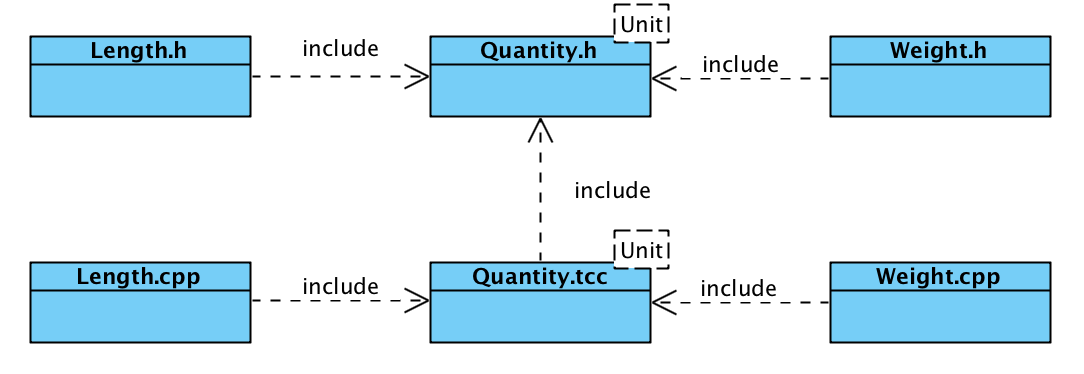
\includegraphics[width=0.8\textwidth]{figures/explict-template-inst.png}
\caption{显式模板实例化} 
 \label{fig:explict-template-inst}
\end{figure}



\begin{advise}
子类化优于\code{typedef}
\end{advise}

如果使用\code{typedef},如果存在对\code{Length}的依赖,即使是名字的声明依赖,除了包含头文件之外,别无选择。

另外,如果\code{Quantity}存在\code{virtual}函数时,\code{Length}还有进一步扩展\code{Quantity}的可能性,从而使设计提供了更大的灵活性。

反例:
\begin{leftbar}
\begin{c++}[caption={\ttfamily{quantity/Length.h}}]
#ifndef TYIW7364_JG6389457_BVGD7562_VNW12_JFH
#define TYIW7364_JG6389457_BVGD7562_VNW12_JFH

#include <quantity/Quantity.h>

struct LengthUnit;
typedef Quantity<LengthUnit> Length;

#endif
\end{c++}
\end{leftbar}

正例:
\begin{leftbar}
\begin{c++}[caption={\ttfamily{quantity/Length.h}}]
#ifndef TYIW7364_JG6389457_BVGD7562_VNW12_JFH
#define TYIW7364_JG6389457_BVGD7562_VNW12_JFH

#include <quantity/Quantity.h>

struct LengthUnit;
struct Length : Quantity<LengthUnit> {};

#endif
\end{c++}
\end{leftbar}

\end{content}

\begin{savequote}[45mm]
\ascii{Controlling complexity is the essence of computer programming.}
\qauthor{\ascii{- Brian Kernighan}}
\end{savequote}

\chapter{不可变性}
\label{ch:immutability}

\section{const}

\begin{content}

\begin{regulation}
使用\ascii{const},或者枚举常量替代\ascii{\#define}的宏常量。
\end{regulation}

这样做可以及大地提高编译时类型的安全性。

\begin{regulation}
当类的成员函数具有查询语义时,应将其声明为\ascii{const}成员函数。
\end{regulation}

此处具有查询语义的函数,泛指所有对对象状态未产生副作用。\ascii{const}成员函数往往都以\ascii{get, is, has,
should}开头。

反例:
\begin{leftbar}
\begin{c++}[caption={cub/math/Rectangle.h}]
#ifndef EWRIUN9037_NVHD6452_JKLSDFUIE7562_HGYE
#define EWRIUN9037_NVHD6452_JKLSDFUIE7562_HGYE

#include <cub/base/BaseTypes.h>

struct Rectangle
{
    Rectangle(U8 width, U8 height);

    U16 calcArea();

private:
    U8 width;
    U8 height;
};

#endif
\end{c++}
\end{leftbar}

此例中未对那些具有查询语义的函数声明为\ascii{const}。\ascii{const}的存在不仅仅是为了提高编译时的安全性检查,更重要的是\ascii{const}建立了用户和类之间的契约关系,并传达了程序员良好设计的心声。

当对象以\ascii{pass-by-const-reference}传递时,用户只能调用其\ascii{const}成员函数;此外,\ascii{const}建立的契约,使\ascii{Replace Temp with Query}的重构手法成为可能。

正例:
\begin{leftbar}
\begin{c++}[caption={math/Rectangle.h}]
#ifndef EWRIUN9037_NVHD6452_JKLSDFUIE7562_HGYE
#define EWRIUN9037_NVHD6452_JKLSDFUIE7562_HGYE

#include <cub/base/BaseTypes.h>

struct Rectangle
{
    Rectangle(U8 width, U8 height);

    U16 calcArea() const;

private:
    U8 width;
    U8 height;
};

#endif
\end{c++}
\end{leftbar}

\begin{advise}
\ascii{const}成员函数不应该修改系统的状态
\end{advise}

编译器只能保证\ascii{const}成员函数修改成员变量时提示错误,而未对修改全局变量,类的静态变量,或者其他的形式的副作用等情况进行检查,应杜绝此类情况的发生。

\begin{regulation}
以\ascii{pass-by-reference-to-const}替代\ascii{pass-by-value}传递对象,以改善性能,并避免切割问题
\end{regulation}

虽然我们不提倡进行过早的优化,但也绝不提倡不成熟的劣化。\ascii{pass-by-reference-to-const}就是此句名言最好的一个例子。

\begin{advise}
当传递内置类型,迭代器及函数对象时,应该\ascii{pass-by-value}。如果使用\ascii{const}修饰,往往可以改善\ascii{API}的可读性。
\end{advise}

其中,\ascii{Status, ActionId}分别是\ascii{U32, U16}的\ascii{typedef},但在设计\ascii{onDone}原型时,\ascii{const}的修饰不仅仅为了改善其安全性,更重要的是与\ascii{TransactionInfo}的\ascii{reference-to-const}形成对称性\footnote{关于对称性,请参考\ascii{Kent
Beck}的著作\ascii{《实现模式》}},改善了\ascii{API}的美感。

反例:
\begin{leftbar}
\begin{c++}[caption={trans-dsl/listener/TransactionListener.h}]
#ifndef UTJKLFJS_467867_NBHD83562_HETRIO_75649
#define UTJKLFJS_467867_NBHD83562_HETRIO_75649

#include <cub/base/Status.h>
#include <cub/trans-dsl/concept/ActionId.h>

struct TransactionInfo;

DEFINE_ROLE(TransactionListener)
{   
    DEFAULT(Status, onStarting(const TransactionInfo&, const ActionId&));
    DEFAULT(Status, onDone(const TransactionInfo&, const ActionId&, const Status&));
};

#endif
\end{c++}
\end{leftbar}

正例:
\begin{leftbar}
\begin{c++}[caption={trans-dsl/listener/TransactionListener.h}]
#ifndef UTJKLFJS_467867_NBHD83562_HETRIO_75649
#define UTJKLFJS_467867_NBHD83562_HETRIO_75649

#include <cub/base/Status.h>
#include <cub/trans-dsl/concept/ActionId.h>

struct TransactionInfo;

DEFINE_ROLE(TransactionListener)
{   
    DEFAULT(Status, onStarting(const TransactionInfo&, ActionId));
    DEFAULT(Status, onDone(const TransactionInfo&, ActionId, Status));
};

#endif
\end{c++}
\end{leftbar}

\begin{regulation}
当返回的是一个新对象时,必须返回其值类型; 更有甚者,返回\ascii{const}的值类型将改善编译时的安全性。
\end{regulation}

反例:
\begin{leftbar}
\begin{c++}[caption={math/Rectangle.h}]
#ifndef EWRIUN9037_NVHD6452_JKLSDFUIE7562_HGYE
#define EWRIUN9037_NVHD6452_JKLSDFUIE7562_HGYE

#include <cub/base/BaseTypes.h>

struct Rectangle
{
    Rectangle(const U8 width, const U8 height);

    U16 getArea() const;
    U16 getPerimeter() const;
    
    bool operator==(const Rectangle& rhs) const;
    bool operator!=(const Rectangle& rhs) const;
    
    Rectangle& operator+=(const Rectangle& rhs) const;
    Rectangle& operator+(const Rectangle& rhs) const;

private:
    const U8 width;
    const U8 height;
};

#endif
\end{c++}
\end{leftbar}

按照惯例,\ascii{operator+}返回的是一个新实例,返回值应该设计为值类型。如果提供\ascii{const}的修饰能够加强编译时的安全性检查。此外,需要注意的是\ascii{operator+=}返回的是修改后的\texttt{*this}对象引用。

正例:
\begin{leftbar}
\begin{c++}[caption={math/Rectangle.h}]
#ifndef EWRIUN9037_NVHD6452_JKLSDFUIE7562_HGYE
#define EWRIUN9037_NVHD6452_JKLSDFUIE7562_HGYE

#include <cub/base/BaseTypes.h>

struct Rectangle
{
    Rectangle(const U8 width, const U8 height);

    U16 getArea() const;
    U16 getPerimeter() const;
    
    bool operator==(const Rectangle& rhs) const;
    bool operator!=(const Rectangle& rhs) const;
    
    Rectangle& operator+=(const Rectangle& rhs) const;
    Rectangle operator+(const Rectangle& rhs) const;

private:
    const U8 width;
    const U8 height;
};

#endif
\end{c++}
\end{leftbar}

\begin{regulation}
不能返回局部对象的引用或指针。
\end{regulation}

返回值类型还是引用类型常常会困扰部分\cpp{}程序员。其实规则非常简单,返回值对象当且仅当需要创建新对象的时候,此时如果企图返回引用或指针,将导致运行时异常。

\end{content}

\section{不可变类}

\begin{content}

\begin{advise}
鼓励设计不可变类\ascii{(Immutable Class)}表达值对象\ascii{(Value Object)}的语义
\end{advise}

不可变类的每一个实例在创建的时候就包含了所有必要的信息,其对象在整个生命周期中都不会发生变化。不可变类具有如下几方面的优势:
\begin{enum}
  \eitem{相对于可变对象的复杂的状态空间,不可变类仅有一个状态,容易设计、实现和控制}
  \eitem{不可变类本质上是线程安全的,它们不需要同步}
  \eitem{不可变类可被自由地共享,重用对象是一种良好设计的习惯}
\end{enum}

设计不可变类,需遵循如下规则:
\begin{enum}
  \eitem{不能提供修改对象状态的方法}
  \eitem{保证类不能被扩展,切忌提供\ascii{virtual destructor}}
  \eitem{所有成员变量和方法都是\ascii{const}}
  \eitem{所有成员变量都是\ascii{private}}
  \eitem{绝不允许重新赋值,但允许克隆出新的实例}
\end{enum}

不可变类唯一的缺点就是,对于每一个不同的值都需要一个单独的对象。当需要创建大量此类对象时,性能可能成为瓶颈。当性能成为关键瓶颈的时候,为不可变类设计可变配套类是一种典型的设计方式。

上例讲解的\ascii{Rectangle}类也是一种典型的不可变类的设计;而\ascii{std::string}为了追求性能,设计为一个可变类。

\begin{regulation}
尽量使类的可变性最小化
\end{regulation}

坚决抵制为每一个\ascii{get}函数都写一个\ascii{set}函数,除非存在一个很好的理由。构造函数的职责就是来完成对象的初始化,并建立起所有的约束关系。除非有很好的理由,不要在构造函数之外提供其他公开的初始化方法。

\end{content}


\begin{savequote}[45mm]
\ascii{Write programs for people first, computers second.}
\qauthor{\ascii{- Steve McConnell}}
\end{savequote}

\chapter{命名} 
\label{ch:naming}

\begin{content}

良好的命名将改善代码的表现力,与其说命名是一门技术,不如说它是一门艺术。必须坚持、并慎重地给程序中的每一个实体取好名字,让其名副其实,代码的可读性将得到极大的改善。

\end{content}

\section{Baby Names}
\begin{content}

\begin{regulation}
遵守统一的命名规范
\end{regulation}

一些程序设计语言,从诞生的时刻就有着自己的文化背景,整个社区有着统一的命名规则。但\cpp{}在社区中存在众多的命名风格,有的与时俱进,也非常人性化;有的则已经与现代软件工程格格不入\footnote{例如社区中依然存在一批忠实的匈牙利的守护者,他们认为一个名称没有前缀和后缀标识它们的类型,他们几乎都看不懂代码了。}。

下文罗列了一些\cpp{}典型的命名规范供参考。每一种命名规范都有自身自己的优缺点,团队应该根据自身的实际情况选择适合自己的命名规范。最重要的是,团队应遵循统一的命名规范,不应该出现两种或两种以上的命名风格。

我们推荐团队使用下文中任意一种命名风格,但如果由于历史遗留原因导致革新非常困难,而无法采用新的命名规范,团队依然要保持统一的命名规范,避免出现多种命名风格。

\begin{table}[!htb]
\resizebox{0.95\textwidth}{!} {
\begin{tabular*}{1.2\textwidth}{@{}ll@{}}
\toprule
\ascii{Identifier} & \ascii{Examples} \\
\midrule
\ascii{Namespace}  & \ascii{std, dcm, mockcpp, testing} \\
\ascii{Class/Struct/Union} & \ascii{Timer, FutureTask, LinkedHashMap, HttpServlet} \\ 
\ascii{Method} & \ascii{remove, ensureCapacity, getCrc} \\
\ascii{Constant/Macro/Enum} & \ascii{IDLE, ACTIVE, MAX\_LINK\_NUM} \\
\ascii{Local Variable} & \ascii{i, xref, houseNumber} \\
\ascii{Type Parameter} & \ascii{T, E, K, V, X, T1, T2} \\
\bottomrule
\end{tabular*}
}
\caption{驼峰命名规范1}
\label{tbl:naming-1}
\end{table}

还有一种命名风格与上一种风格类同,只是成员函数/函数都以大写开头的驼峰命名。

\begin{table}[!htb]
\resizebox{0.95\textwidth}{!} {
\begin{tabular*}{1.2\textwidth}{@{}ll@{}}
\toprule
\ascii{Identifier} & \ascii{Examples} \\
\midrule
\ascii{Namespace}  & \ascii{std, dcm, mockcpp, testing} \\
\ascii{Class/Struct/Union} & \ascii{Timer, FutureTask, LinkedHashMap, HttpServlet} \\ 
\ascii{Method} & \ascii{Remove, EnsureCapacity, GetCrc} \\
\ascii{Constant/Macro/Enum} & \ascii{IDLE, ACTIVE, MAX\_LINK\_NUM} \\
\ascii{Local Variable} & \ascii{i, xref, houseNumber} \\
\ascii{Type Parameter} & \ascii{T, E, K, V, X, T1, T2} \\
\bottomrule
\end{tabular*}
}
\caption{驼峰命名规范2}
\label{tbl:naming-2}
\end{table}


第三种命名风格,主要体现在标准库或\ascii{Boost}准标准库社区,其规则非常简单,下划线分割的全小写,或下划线分割的全大写。

\begin{table}[!htb]
\resizebox{0.95\textwidth}{!} {
\begin{tabular*}{1.2\textwidth}{@{}ll@{}}
\toprule
\ascii{Identifier} & \ascii{Examples} \\
\midrule
\ascii{Namespace}  & \ascii{boost, details, mpl} \\
\ascii{Class/Struct/Union} & \ascii{any, is\_enum, shared\_ptr} \\ 
\ascii{Method} & \ascii{any\_cast, type\_of} \\
\ascii{Constant/Macro/Enum} & \ascii{IDLE, ACTIVE, MAX\_LINK\_NUM} \\
\ascii{Local Variable} & \ascii{i, xref, house\_number} \\
\ascii{Type Parameter} & \ascii{T, E, K, V, X, T1, T2} \\
\bottomrule
\end{tabular*}
}
\caption{标准库或\ascii{boost}命名规范}
\label{tbl:naming-3}
\end{table}

\begin{regulation}
绝不使用汉语拼音命名
\end{regulation}

必须实用标准的英语命名程序实体,不允许实用汉语拼音。

\begin{regulation}
类名应该是名词或名词短语;接口可以是形容词; 方法名应该是动词或动词短语
\end{regulation}

\begin{table}[!htb]
\resizebox{0.95\textwidth}{!} {
\begin{tabular*}{1.2\textwidth}{@{}ll@{}}
\toprule
\ascii{类别} & \ascii{举例} \\
\midrule
\ascii{正确的类名}  & \ascii{AddressParser, EventRegistry} \\
\ascii{错误的类名} & \ascii{ParseAddress, RegisterEvent} \\
\bottomrule
\end{tabular*}
}
\caption{类名}
\label{tbl:naming-4}
\end{table}

接口可以是形容词,最为常见的就是定义能力接口,即以\ascii{-able}结尾。

反例:
\begin{leftbar}
\begin{c++}[caption={\ttfamily{cub/thread/Runnable.h}}]
#ifndef LJKYIUERUIQ09857983_NVHKJKHA86100494_JGYQPIPWNC
#define LJKYIUERUIQ09857983_NVHKJKHA86100494_JGYQPIPWNC

#include <cub/base/Keywords.h>

// 接口必须是形容词或名词,不允许是动词
DEFINE_ROLE(Run)
{
    ABSTRACT(void run());
};

#endif
\end{c++}
\end{leftbar}

正例:
\begin{leftbar}
\begin{c++}[caption={\ttfamily{cub/thread/Runnable.h}}]
#ifndef LJKYIUERUIQ09857983_NVHKJKHA86100494_JGYQPIPWNC
#define LJKYIUERUIQ09857983_NVHKJKHA86100494_JGYQPIPWNC

#include <cub/base/Keywords.h>

DEFINE_ROLE(Runnable)
{
    ABSTRACT(void run());
};

#endif
\end{c++}
\end{leftbar}

\begin{regulation}
如果函数返回值为\ascii{bool},加上\ascii{is, has, can, should, need}将会增强语意
\end{regulation}

反例:
\begin{leftbar}
\begin{c++}
bool readPassword = true;
\end{c++}
\end{leftbar}

至少存在两种解释,

\begin{enum}
  \eitem{\ascii{We need to read the password}}
  \eitem{\ascii{The password has already been read}}
\end{enum}

正例:
\begin{leftbar}
\begin{c++} 
bool needPassword = true;
bool userIsAuthenticated = true; 
\end{c++}
\end{leftbar}

\begin{regulation}
丰富你的单词库,在面对具体问题时你具有更多的\ascii{Colorfull Words}
\end{regulation}

如\reftbl{colorful-words}所示,同一概念是有很多种表达方式的。

\begin{table}[!htb]
\resizebox{0.95\textwidth}{!} {
\begin{tabular*}{1.2\textwidth}{@{}ll@{}}
\toprule
\ascii{Word} & \ascii{Alternatives} \\
\midrule
\ascii{send}  & \ascii{deliver, dispatch, announce, distribute, route} \\
\ascii{find} & \ascii{dsearch, extract, locate, recover} \\ 
\ascii{start} & \ascii{launch, create, begin, open} \\
\ascii{make} & \ascii{create, set up, build, generate, compose, add, new} \\
\bottomrule
\end{tabular*}
}
\caption{丰富的词汇}
\label{tbl:colorful-words}
\end{table}

\begin{regulation}
名字在明确意图的前提下越短越好
\end{regulation}

反例:
\begin{leftbar}
\begin{c++}
ControllerForEfficientHandlingOfStrings
ControllerForEfficientStorageOfStrings
\end{c++}
\end{leftbar}

因为这两个类名实在是太相似了,一时间很难区分。当别人打算复用你的代码时,必然承受着巨大的记忆包袱。

另外,实体名称的长度应该于作用域的大小成正比。如果是一个实体暴露在全局命名空间,则需要适当增加名字长度,防止名字冲突\footnote{应该使用命名空间,避免增加模块前缀信息。}。相反地,在一个很小的函数之内可见的局部变量,尤其在一个短小的\ascii{for}循环作用域内,完全没有必要取一个很长的名字。

反例:
\begin{leftbar}
\begin{c++}[caption={\ttfamily{cub/trans-dsl/listener/MutilEventListener.cpp}}]
void MutilEventListener::onEventDone()
{
    for(int index=0; index!=listeners.size(); index++)
    {
        listeners[index].onEventDone();
    }
}
\end{c++}
\end{leftbar}

优秀的程序员在命名的长短的取舍总是游刃有余,但从来没有降低过代码的意图。

正例:
\begin{leftbar}
\begin{c++}[caption={\ttfamily{cub/trans-dsl/listener/MutilEventListener.cpp}}]
void MutilEventListener::onEventDone()
{
    for(int i=0; i!=listeners.size(); i++)
    {
        listeners[i].onEventDone();
    }
}
\end{c++}
\end{leftbar}

使用\ascii{C++11}的\ascii{for-each}特性,可进一步改善设计。

正例:
\begin{leftbar}
\begin{c++}[caption={\ttfamily{cub/trans-dsl/listener/MutilEventListener.cpp}}]
void MutilEventListener::onEventDone()
{
    for(auto& listener : listeners)
    {
        listeners.onEventDone();
    }
}
\end{c++}
\end{leftbar}


\begin{regulation}
程序中每个实体都应该有一个意图明确\ascii{(Intention-Revealing)}的名称
\end{regulation}

反例:
\begin{leftbar}
\begin{c++}[caption={\ttfamily{game/chess/GameBoard.h}}]
vector<vector<int> > getThem() 
{
    vector<vector<int> > list1;
    
    for(auto x : theList)
    {
        if(x[0] == 4)
        {   
            list1.add(x);
        }
    }
    
    return list1;
}
\end{c++}
\end{leftbar}

\begin{enum}
  \eitem{\ascii{vector<vector<int> >}的语法令人抓狂}
  \eitem{\ascii{getThem}让人看不清楚它的本意}
  \eitem{\ascii{theList}到底是什么东西?}
  \eitem{\ascii{0}下标意味着什么?\ascii{4}又意味着什么?}
  \eitem{\ascii{list1}就是为了编译通过吗?}
\end{enum}

换一个好名字之后,并对数据结构的实现细节进行了简单的封装,便可以得到一个更合理的设计。

正例:
\begin{leftbar}
\begin{c++}[caption={\ttfamily{game/chess/Cell.h}}]
#ifndef UTJKLFJS_467867_NBHD83562_HETRIO_75649
#define UTJKLFJS_467867_NBHD83562_HETRIO_75649

#include <vector>

struct Cell
{
    bool isFlagged() const;

private:
    std::vector<int> states;
};

using Cells = std::vector<Cell>;

#endif
\end{c++}
\end{leftbar}

\begin{leftbar}
\begin{c++}[caption={\ttfamily{game/chess/GameBoard.h}}]
#ifndef JAAA_1295_BBVBAA_GFYQQPPAAMZZ0092444_N
#define JAAA_1295_BBVBAA_GFYQQPPAAMZZ0092444_N

#include <game/chess/Cell.h>

struct GameBoard
{
    void collectFlaggedCells(Cells&) const;

private:
    Cells board;
};

#endif
\end{c++}
\end{leftbar}

\begin{leftbar}
\begin{c++}[caption={\ttfamily{game/chess/GameBoard.cpp}}]
void GameBoard::collectFlaggedCells(Cells& cells) const
{
    for(auto &cell : board)
    {
        if(cell->isFlagged())
        {
            cells.push_back(cell);
        }
    }
}  
\end{c++}
\end{leftbar}
\end{c++}
\end{leftbar}

\begin{regulation}
避免在名称中携带数据结构的信息
\end{regulation}

\begin{content}

别用\ascii{accountList,accountArray}指定一组账号,当包含\ascii{Account}的容器不在是一个\ascii{List}或\ascii{Array}的时候,就会引发错误的判断。所以,用\ascii{accountGroup},\ascii{bunchOfAccounts},甚至直接使用\ascii{accounts},情况都会更好一些。

\end{content}

\begin{regulation}
\ascii{Noise Words are Redundant},消除噪声后将得到一个更加精准的名字
\end{regulation}

\begin{table}[!htb]
\resizebox{0.95\textwidth}{!} {
\begin{tabular*}{1.2\textwidth}{@{}ll@{}}
\toprule
\ascii{Short Name} & \ascii{Redundant Names} \\
\midrule
\ascii{Name}  & \ascii{StrName, NameString} \\
\ascii{Customer} & \ascii{CustmerObject, CustmerInfo} \\ 
\ascii{accouts} & \ascii{accountList, accountArray} \\
\ascii{accout} & \ascii{accountData, accountInfo} \\  
\ascii{money} & \ascii{moneyAmount} \\
\ascii{message} & \ascii{theMessage} \\
\bottomrule
\end{tabular*}
}
\caption{消除冗余的噪声}
\label{tbl:redundant-words}
\end{table}

\begin{regulation}
使用\ascii{Domain}领域内的名称,将更直白地表明你的设计,增强领域内成员的沟通
\end{regulation}

\begin{enum}
  \eitem{\ascii{Factory, Visitor, Repository}}
  \eitem{\ascii{valueOf, of, getInstance, newInstance, newType}}
  \eitem{\ascii{AppendAble, Closeable, Runnable, Readable, Invokable}}
\end{enum}

\begin{content}

当使用\ascii{Visitor},你在使用访问者模式;当使用\ascii{valueOf,
of},你在使用静态工厂方法。领域内的命名风格,让领域内的成员更加快捷地理解你的设计意图。

\end{content}

\end{content}

\section{匈牙利命名}
\begin{content}

\begin{advise}
摒弃匈牙利命名
\end{advise}

匈牙利命名曾风靡一时。但是,现代编程语言具有更丰富的类型系统;人们更趋于使用更小的类,更短的函数,让每一个变量定义都在可控的视野范围之内;此外,\ascii{IDE}变得越来智能和强大,匈牙利命名反而变成了一种噪声和肉刺。

\begin{advise}
摒弃给成员变量加前缀,或后缀。
\end{advise}

为类的成员变量增加\ascii{m\_}前缀同样没有必要。与其纠结加前缀还是不加前缀,不如花费更多的时间将类分解;当类足够小,职责足够单一,加之现代\ascii{IDE}的着色功能,成员变量和普通变量一眼便能识别开来\footnote{\ascii{Eclipse}默认使用蓝色与普通变量区别开来,其他\ascii{IDE}也提供类似的功能。}。

\begin{advise}
摒弃常量的前缀。
\end{advise}

常量前增加\ascii{k\_}前缀同样没有必要,如果熟悉了大写、下划线隔开的命名风格,\ascii{k\_}前缀完全属于多余。

\begin{advise}
摒弃接口和类的前缀
\end{advise}

在接口前增加\ascii{I\_},在类前增加\ascii{C\_},同样完全没有必要,它只能对重构带来阻力,百害而无一利。

反例:
\begin{leftbar}
\begin{c++}[caption={\ttfamily{trans-dsl/sched/IAction.h}}]
#ifndef NVCHKJSD903085_JGOIUUE906894_VBKSJKJA075774
#define NVCHKJSD903085_JGOIUUE906894_VBKSJKJA075774    

#include <cub/base/Keywords.h>
#include <cub/base/Status.h>

struct TransactionInfo;

DEFINE_ROLE(IAction)
{
    ABSTRACT(Status exec(const TransactionInfo&));
};

#endif
\end{c++}
\end{leftbar}

正例:
\begin{leftbar}
\begin{c++}[caption={\ttfamily{trans-dsl/sched/IAction.h}}]
#ifndef NVCHKJSD903085_JGOIUUE906894_VBKSJKJA075774
#define NVCHKJSD903085_JGOIUUE906894_VBKSJKJA075774    

#include <cub/base/Keywords.h>
#include <cub/base/Status.h>

struct TransactionInfo;

DEFINE_ROLE(Action)
{
    ABSTRACT(Status exec(const TransactionInfo&));
};

#endif
\end{c++}
\end{leftbar}

如果非得在接口与实现中选择,宁愿选择实现中增加\ascii{Impl}后缀。

\end{content}

\begin{savequote}[45mm]
\ascii{On the other hand, we cannot ignore efficiency.}
\qauthor{\ascii{– Jon Bentley}}
\end{savequote}

\chapter{注释} 
\label{ch:comment}

\section{注释}
\begin{content}

\begin{regulation}
注释不如花费更多时间给实体取一个好名字,让其名副其实。
\end{regulation}

反例:
\begin{leftbar}
\begin{c++}
int time; // elapsed time in days
\end{c++}
\end{leftbar}

正例:
\begin{leftbar}
\begin{c++}
int elapsedTimeInDays;
\end{c++}
\end{leftbar}

注释应成为一种羞耻的活动,当需要添加注释的时候,往往是改善设计的最好时机。

\begin{regulation}
注释符号与注释内容之间要用一个空格分割。
\end{regulation}

当注释内容与注释符号之间没有空格,尤其是中文注释,导致部分编译器词法分析错误,导致编译失败。

反例:
\begin{leftbar}
\begin{c++}
/*multi-line comment*/
//sigle-line comment
\end{c++}
\end{leftbar}

正例:
\begin{leftbar}
\begin{c++}
/* multi-line comment */
// single-line comment
\end{c++}
\end{leftbar}

\begin{regulation}
消除所有没有必要的注释
\end{regulation}

没有携带任何信息量的注释都是没有必要的。如下列的注释,维护它简直就是一种巨大的包袱,有时候它的存在就像一个笑话。

反例:
\begin{leftbar}
\begin{c++}
/**
 * Constructor
 */
InvokedAtMost(const unsigned int times);

/**
 * @param Invocation
 * @return bool
 */
bool matches(const Invocation& inv) const;
\end{c++}
\end{leftbar}

\begin{regulation}
消除所有误导性、过时的、与设计实现不匹配的注释
\end{regulation}

如果注释和代码已经失去匹配,意图甚至是相反的。这样的注释如果继续存在,贻害的肯定不止一个人。“假如代码和注释不一致,那么很可能两者都是错误的”,\ascii{Norm Schryer}形象地描述了不一致的注释给代码维护者带来的困扰。

\begin{regulation}
消除所有日志型、归属、签名的注释
\end{regulation}

修正一个\ascii{bug}时,都需要在函数头的注释表中记录被次修改的内容。放弃这种“好”习惯吧,请将这些详细的信息提交给源代码控制系统,那里是此类注释最好的归所。

\begin{regulation}
消除所有\ascii{//end if, //end while, //end for, // end try}的注释
\end{regulation}

因为逻辑太过于冗长、复杂,又为了增强可读性,往往在花括号后面标记\ascii{//end if, //end while, //end for, // end try},这往往是简化表达式、提取函数的最佳时机。

\begin{regulation}
已经被注释掉的代码,应该立即删除
\end{regulation}

不要珍惜这些冗余的代码,害怕丢掉这些代码而买不到后悔药。你要相信,从源代码控制系统中追回这份被删除的代码易如反掌。

\begin{regulation}
在需要注释的时候,一定要加注释
\end{regulation}

因公司版权的保护,需要增加版权法律信息注释\footnote{发布开源代码时,也常常需要增加必要的\ascii{GNU, BSD等}公共许可证}。幸运的是,这类问题可以通过代码模板轻松解决,不会成为造成程序员的任何负担。

在已经尽全力也无法用代码表述清楚时,增加必要的注释会使代码更加容易被别人理解和维护。在这些场景下,注释将成为我们最后一根救命稻草。

\begin{enum}
  \eitem{代码无法明确的意图也需要增加注释}
  \eitem{如果在代码中存在特殊的陷阱、实现手法等情况,此时注释变得尤为宝贵}
\end{enum}

例如,当操作复杂的位运算时,提供比特位的内存映像的注解,将有利于加快读者阅读代码的速度。

正例:
\begin{leftbar}
\begin{c++}
// Fast version of "hash = (65599 * hash) + c"
hash = (hash << 6) + (hash << 16) - hash + c;
\end{c++}
\end{leftbar}

当定义难以理解的正则表达式时,提供更直观的格式说明,同样可以改善对代码的理解。

正例:
\begin{leftbar}
\begin{c++}
// kk::mm::ss, MM dd, yyyy
std::string timePattern = "\\d{2}:\\d{2}:\\d{2}, \\d{2} \\d{2}, \\d{4}";
\end{c++}
\end{leftbar}

\end{content}
\begin{savequote}[45mm]
\ascii{Do the simplest thing that could possibly work.}
\qauthor{\ascii{- Kent Beck}}
\end{savequote}

\chapter{简化逻辑}
\label{ch:simple-logic}

\section{简化控制逻辑}

\begin{content}

\begin{advise}
\ascii{YODA Notation}已经是过去时
\end{advise}

\begin{leftbar}
\begin{c++}
if (length <= MAX_STREAM_LEN)
\end{c++}
\end{leftbar}

要比

\begin{leftbar}
\begin{c++}
if (MAX_STREAM_LEN >= length)
\end{c++}
\end{leftbar}

更具有表达力。再看一个例子,

\begin{leftbar}
\begin{c++}
while (bytesReceived < bytesExpected)
\end{c++}
\end{leftbar}

要比

\begin{leftbar}
\begin{c++}
while (bytesExpected > bytesReceived)
\end{c++}
\end{leftbar}

更具由表达力。因为前者更加符合人类的思维,或这说更符合英语的表达习惯,\ascii{"if you are at least 18 years old."}明显比\ascii{"if 18 years is less than or equal to your age"}更加符合英语表达习惯。是的,英语更加习惯将稳定的一侧放在右边\ascii{(right-hand side)}。

但是,在\clang{}或者\cpp{}语言中,如果\ascii{==}被误用为\ascii{=},则可能发生副作用的危险,而且编译时并不能做到安全的检查,从而产生了严重的\ascii{bug}。

\begin{leftbar}
\begin{c++}
// 缺少等号,造成严重的运行时错误
if (ptr = NULL)
\end{c++}
\end{leftbar}

幸运的是,现代编译器对此类误用通常报告警告信息;如果保持\ascii{TDD}开发节奏,小步前进,此类低级错误很难逃出测试的法网。

正例:
\begin{leftbar}
\begin{c++}
if (ptr == NULL)
\end{c++}
\end{leftbar}

反例:
\begin{leftbar}
\begin{c++}
if (NULL == ptr)
\end{c++}
\end{leftbar}


\begin{regulation}
在简单逻辑的情况下,鼓励使用\ascii{?:}三元表达式;但是,当表达式变得非常复杂时,\ascii{if-else}可能是更好的选择
\end{regulation}

反例:
\begin{leftbar}
\begin{c++}
if (hour >= 12) 
{
    time += "pm";
} 
else 
{
    time += "am";
}
\end{c++}
\end{leftbar}

正例:
\begin{leftbar}
\begin{c++}
time_str += (hour >= 12) ? "pm" : "am";
\end{c++}
\end{leftbar}

但很多程序员往往因为习惯了\ascii{if-else}而忽视了这种简洁的表达式。但是,当表达式变得非常复杂时,\ascii{if-else}可能是更好的选择。

反例:
\begin{leftbar}
\begin{c++}
return exponent >= 0 ? mantissa * (1 << exponent) : mantissa / (1 << -exponent);
\end{c++}
\end{leftbar}

正例:
\begin{leftbar}
\begin{c++}
if (exponent >= 0)
{
    return mantissa * (1 << exponent);
}
else
{
    return mantissa / (1 << -exponent);
}
\end{c++}
\end{leftbar}

\begin{regulation}
当逻辑表达式已经具有\ascii{true或false}语义时,则无需显示地加上\ascii{true或false}
\end{regulation}

反例:
\begin{leftbar}
\begin{c++}
bool exist = nodes.contains(NodeId(2)) ? true : false;
if(exist == true)
{
    ...
}
\end{c++}
\end{leftbar}

正例:
\begin{leftbar}
\begin{c++}
if(nodes.contains(NodeId(2))
{
    ...
}
\end{c++}
\end{leftbar}

\begin{regulation}
避免函数嵌套过深,擅用卫语句从函数中提前返回,或从嵌套的语句中提前返回;但绝对不滥用\ascii{break, continue}
\end{regulation}

嵌套过深的函数,将迫使读者跟踪运行时\ascii{stack},同样给读者增加过重的记忆包袱。

反例:
\begin{leftbar}
\begin{c++}
if (userResult == SUCCESS)
{
    if (permissionResult != SUCCESS)
    {
        reply.writeError(permissionResult);
        return;
    }
    reply.writeError("");
}
else
{
    reply.writeError(usrResult);
}
\end{c++}
\end{leftbar}

正例:
\begin{leftbar}
\begin{c++}
if (userResult != SUCCESS)
{
    reply.writeError(usrResult);
    return;
}

if (permissionResult != SUCCESS)
{
    reply.writeError(permissionResult);
    return;
}

reply.writeError("");

\end{c++}
\end{leftbar}

虽然在代码阅读过程中\ascii{break, continue,
return}常常打断了人的思维。但在函数短小,意图明确的情况下,\ascii{break, continue,
return}相反能给人一种“跳过此项”的特殊意图,代码嵌套逻辑得到了改善。

\begin{regulation}
擅用解释型变量,或提供意图明确的、内联的提取函数
\end{regulation}

解释型变量,或提取函数的重构手法有利于改善代码的可读性,往往后者更具有表达力。

反例:
\begin{leftbar}
\begin{c++}
if (line.split(":")[0].trim() == "root")
\end{c++}
\end{leftbar}

正例:
\begin{leftbar}
\begin{c++}
String userName = line.split(":")[0].trim();
if (userName == "root")
{
    ...
}
\end{c++}
\end{leftbar}

\ascii{split}函数将字符串按照指定的正则表达式进行拆分,并提供一个良好的意图变量,将大大改善逻辑的清晰度。

\begin{regulation}
将局部变量的作用域最小化
\end{regulation}

这条规则可能对从\clang{}转变过来的\cpp{}程序员更有指导意义,但改变这样的陋习可能需要一些适应的时间。例如局部于\ascii{for}的循环变量,当它的使命完成之后,应立即销毁它,避免这个变量被再次使用的风险。

\begin{leftbar}
\begin{c++}
map<string, string> addressBook;
for (auto &entry : addressBook) 
{ 
    std::cout << entry->first << "," << entry->second << std::endl;
}
\end{c++}
\end{leftbar}

\end{content}

\begin{savequote}[45mm]
\ascii{I'm not a great programmer; I'm just a good programmer with great habits.}
\qauthor{\ascii{- Kent Beck}}
\end{savequote}

\chapter{类设计}
\label{ch:class-design}

%%%%%%%%%%%%%%%%%%%%%%%%%%%%%%%%%%%%%%%%%%%%%%%%%%%%%%%%%%%%%%%%%%%%%%%%%%%%%%%%
\section{构造与析构}

\begin{content}

\begin{regulation}
抵制设计和实现上帝类
\end{regulation}

上帝类是一种典型的代码坏味道,程序员几乎都曾经历过被巨类所困扰的经历。\ascii{20-30}多个成员变量在成员函数中穿梭,犹如像全局变量一样难理解和控制。此外,修改这个巨类需要高超的技能,因为你根本不确定代码的修改是否会影响其他的东西。

消除这样的巨类,关键是识别出类中的主要职责,按照\ascii{SRP}原则来分解巨类,将类拆分成为一个个细小粒度的、高度可复用的、可组合的小类\footnote{详细内容可参考\ascii{Michael C. Feathers}所著的\ascii{《Working Effectively with Legacy Code》}}。

\begin{regulation}
明确\cpp{}的初始化规则
\end{regulation}

初始化永远是程序员心中的痛,抛开一些不重要的细节,其实\cpp{}语言的初始化规则非常简单。\cpp{}使用构造函数完成类初始化,而构造函数使用初始化列表完成初始化的工作。初始化列表首先调用父类的构造函数,然后按照类中定义的的成员变量的顺序依次进行初始化。

没有显式地调用父类构造函数,编译器则自动调用父类的默认构造函数;如果对应的父类没有默认构造函数,则需显式地调用特定的带参构造函数,否则编译失败。

依次类推,如果没有显式地调用成员变量的构造函数,则编译器自动地调用成员变量的默认构造函数;如果对应的成员变量没有默认构造函数,则需显式地调用特定的带参构造函数,否则编译失败。

一般地,如果已经明确需要调用默认构造函数,为了消除冗余代码,则无需显式地进行调用。

特殊地,const数据成员,引用数据成员必须在初始化列表中进行初始化。

\begin{regulation}
在初始化列表中显式地初始化所有内置数据类型的成员变量,\cpp{}语言并没有保证其初始化
\end{regulation}

基本数据类型包括整形,浮点型,指针,引用等类型。当设计一个含有基本数据类型的成员变量时,必须定义构造函数完成所有成员变量的初始化。

\ascii{TransData}必须实现对基本数据类型的成员变量的初始化,否则行为未定义。至于泛型类型\ascii{T}则要求必须存在默认构造函数,否则编译失败。

\begin{leftbar}
\begin{c++}[caption={\ttfamily{cub/base/TransData.h}}]
#ifndef JLGOUIW12975_VBATQ75656_YRTQKS897564_NVGSSJ
#define JLGOUIW12975_VBATQ75656_YRTQKS897564_NVGSSJ

template<typename T>
struct TransData
{
   TransData();
   ~TransData();

   void confirm()
   void revert()

private:
   T values[2];
   unsigned char valid :1;
   unsigned char memoed :1;
   unsigned char unstable :1;
   unsigned char current :1;
   unsigned char :4;
};

template<typename T>
TransData<T>::TransData()
  : valid(0), memoed(0), unstable(0), current(0)
{
}

#endif
\end{c++}
\end{leftbar}

\begin{regulation}
在初始化列表中,而非在构造函数体内进行初始化
\end{regulation}

如果类类型的成员变量没有在初始化列表中进行初始化,事实上编译器调用的是默认构造函数(如果没有默认构造函数,需要显式地调用带参构造函数;否则编译错误)。

这里需要明确地区分初始化与赋值的语义。如果将类类型的初始化放在构造函数体内,则编译器首先在初始化列表中调用默认构造函数,然后再在其构造函数体内调用\ascii{operator=}重新赋值。这样的行为往往是低效的,不是我们所期望的初始化行为。

\begin{regulation}
初始化列表顺序与成员变量定义的顺序保持一致
\end{regulation}

因为编译器的初始化是按照类中成员变量的声明顺序依次进行初始化,如果违背这个规则,可能出现初始化顺序依赖的问题。

\begin{regulation}
除非确认编译器能够正确地调用对应父类或成员变量的默认构造函数,并符合预期行为;否则需要显式地调用其带参构造函数完成初始化
\end{regulation}

相反地,如果已经确认编译器能够正确地调用对应父类或成员变量的默认构造函数,并符合预期行为,无需再显示地调用其默认构造函数,否则将产生冗余的代码。

\begin{regulation}
使用\ascii{RAII}完成资源的安全管理
\end{regulation}

\ascii{RAII(Resource acquisition is initialization)}是一种有用的技术,可实现了资源的安全管理功能。

\begin{leftbar}
\begin{c++}[caption={\ttfamily{cub/thread/Lock.h}}]
#ifndef ITUYIYJL9_067251067_MLBNHKEIOYADMPUO0_NVAXZ
#define ITUYIYJL9_067251067_MLBNHKEIOYADMPUO0_NVAXZ

#include <cub/thread/mutex.h>

struct Lock
{
    Lock(Mutex &mutex) : mutex(mutex)
    {
        mutex.lock();
    }

    ~Lock() 
    {
        mutex.unlock();
    }

private:
    Mutex& mutex;
};

#define SYNCHRONIZED(mutex) Lock mutex##_lock(mutex)

#endif
\end{c++}
\end{leftbar}

\ascii{RAII}利用了局部对象的自动销毁的机制,实现资源的自动释放的功能。

\begin{leftbar}
\begin{c++}[caption={\ttfamily{cub/thread/BlockQueue.h}}]
#ifndef TYOQAMGH2975639_NGGQAOZPY96493950_GFRQA0954
#define TYOQAMGH2975639_NGGQAOZPY96493950_GFRQA0954
    
template<typename T>
void BlockQueue<T>::push(const T& item)
{
    SYNCHRONIZED(mutex);

    // others
}

#endif
\end{c++}
\end{leftbar}

\begin{advise}
在特定场景下延迟初始化对象
\end{advise}

在延迟初始化之前,必须预先占有对象所需要的原始内存空间。但被延迟的对象类型如果在如下两种场景,则无法预先占有原始内存。

\begin{enum}
  \eitem{\ascii{union}内部的放置了非\ascii{POD}类型\footnote{\cpp{}\ascii{11}已经增强了\ascii{union}的语义,\ascii{union}内可放置非\ascii{POD}类型的成员变量了。}}
  \eitem{被延迟初始化的对象无默认构造函数可调用}
\end{enum}

一般地,可以通过定义默认构造函数预先占用好对象内存的空间,当延迟初始化时再重新赋予新的值。但这完全不符合延迟初始化的概念,延迟初始化目标就是为了完全避免这次无谓的默认构造的开销。

可以引入类\ascii{Placement},完成内存的预先占用,当延迟初始化发生时,在此\ascii{Placement}的原始内存上调用\ascii{placement new}完成对象的延迟构造;并在此原始内存上提供了一层直观的、人性化的操作接口,从而可以很方便地操作被修饰的类型\ascii{T}对象。

\begin{leftbar}
\begin{c++}[caption={\ttfamily{cub/base/Placement.h}}]
#ifndef LKSDFLKE95794_HGYETQ1240NBAZUTY75444_MGHHHH
#define LKSDFLKE95794_HGYETQ1240NBAZUTY75444_MGHHHH

#include <string.h>
#include <new>

template <typename T>
struct Placement
{
    void* alloc()
    {
        ::memset(u.buff, 0x00, sizeof(T));
        return u.buff;
    }

    void dealloc()
    {
        getObject()->~T();
    }    

    T* operator->() const
    {
        return (T*)u.buff;
    }

    T& operator*() const
    {
        return *(T*)u.buff;
    }

    T* getObject() const
    {
        return (T*)u.buff;
    }

private:
    union
    {
        char   c;
        short  s;
        int    i;
        long   l;
        float  f;
        double d;
        void*  p;

        char buff[sizeof(T)];
    }u;
};

#endif
\end{c++}
\end{leftbar}

我们分别看两个例子。第一个例子,如果存在两个非\ascii{POD}类型,它们被放在\ascii{union}中,只有在延迟初始化时才能决定其真正的类型的构造。

\begin{leftbar}
\begin{c++}[caption={\ttfamily{money/AccountFactory.h}}]
#ifndef QTA85648888_BFGSE9980666_NNNN_YERQ111_AAAA
#define QTA85648888_BFGSE9980666_NNNN_YERQ111_AAAA

#include <cub/base/BaseTypes.h>

struct Account;

struct AccountFactory
{
    static Account* create(const U8 type);
};

#endif
\end{c++}    
\end{leftbar}

\begin{leftbar}
\begin{c++}[caption={\ttfamily{money/AccountFactory.cpp}}]
#include <money/LocalAccount.h>
#include <money/RemoteAccount.h>
#include <new>

namespace
{
    union AccountMemery
    {
        Placement<LocalAccount>  local;
        Placement<RemoteAccount> remote;
    } m;
}

Account* AccountFactory::create(const U8 type)
{
    switch(type)
    {
    case LOCAL_ACCOUNT: 
        return new (m.local.alloc()) LocalAccount;
    case REMOTE_ACCOUNT: 
        return new (m.remote.alloc()) RemoteAccount;
    default: break;
    }
    
    return 0;
}
\end{c++}    
\end{leftbar}

如果一个类包含一个类类型的数组,除非提供数组元素类型的默认构造函数,否则编译失败。使用\ascii{Placement}预先占用数组所需的内存,再在合适的时机再进行延迟初始化,则可以避免了数组元素的默认构造,提升了效率}。

\begin{leftbar}
\begin{c++}[caption={\ttfamily{sensor/SensorRepository.h}}]
#ifndef MMMM_66310_JFLA98301OQG7492_MFFAZXXX_RREE
#define MMMM_66310_JFLA98301OQG7492_MFFAZXXX_RREE
    
#include <cub/base/Placement.h>
#include <sensor/Sensor.h>
    
struct SensorRepository
{
    SensorRepository() : num(0)
    {}
    
    ~SensorRepository()
    {
        for(U16 i=0; i<num; i++)
        {
            sensors[i].free();
        }
    }

    void addSensor(const U8 id)
    {
        if(num < MAX_NUM_SENSOR)
        {
            new (sensors[num++].alloc()) Sensor(id);
        }
    }
      
private:
    enum { MAX_NUM_SENSOR = 1024 };
    
    U16 num;
    Placement<Sensor> sensors[MAX_NUM_SENSOR];
};

#endif
\end{c++}    
\end{leftbar}

有了\ascii{Placement},此时\ascii{Sensor}就没有必要定义默认构造函数,在延迟初始化的时调用真正的带参构造函数。

\begin{regulation}
绝不\ascii{public}内部的成员变量
\end{regulation}

如果公开了内部成员变量,则违背了信息隐藏机制,这是一种典型的坏味道。相反地,当遇到需要操作遗留系统中\clang{}语言的结构体,需要对其进行封装,并提供相应的成员函数,让其更加符合面向对象的思维。

\begin{leftbar}
\begin{c++}[caption={\ttfamily{cub/base/StructWrapper.h}}]
#ifndef IIU11905749_BVFATQ1_NGFJE8563MCVYYYQQQ_NFG666
#define IIU11905749_BVFATQ1_NGFJE8563MCVYYYQQQ_NFG666
    
template <typename From, typename To>
struct StructWrapper : protected From
{
    static const To& by(const From& from)
    {
        return (const To&)from;
    }
    
    static To& by(From& from)
    {
        return (To&)from;
    }
};

#define STRUCT_WRAPPER(To, From) struct To : StructWrapper<From, To>

#endif
\end{c++}
\end{leftbar}

使用\ascii{StructWrapper}提供的静态工厂方法\ascii{by},可方便地实现\clang{}结构体转变为封装了的\cpp{}类。

%\begin{regulation}
%遇到多个构造器参数时考虑用构建器
%\end{regulation}

\begin{advise}
考虑使用静态工厂方法代替构造函数
\end{advise}

\ascii{static factory method}具有很多优势,
\begin{enum}
  \eitem{\ascii{具有比构造函数更丰富的名称}}
  \eitem{\ascii{不必每次调用时都创建一个对象,实现对象复用,提升性能}}
  \eitem{\ascii{返回类型为接口类型,遵循按接口编程的良好设计原则}}
\end{enum}

以实现对美元、美分打印的为例来讲解\ascii{static factory method}的使用。注意美元的符号在前,而美分的符号在后。
\begin{enum}
  \eitem{\ascii{532 dollars => \$532}}
  \eitem{\ascii{1030 cents => 1030¢}}
\end{enum}

在面对这个问题时,抽象出了\ascii{UsdUnit}类,并提供两个\ascii{static factory method},以实现对\ascii{UsdUnit}实例生成的控制,并通过宏定义改善了\ascii{API}的可读性和方便性。

\begin{leftbar}
\begin{c++}[caption={\ttfamily{money/UsdUnit.h}}]
#ifndef GGG612990097_BSAWQQQQ_NFGGG_VXXZZZ_76555
#define GGG612990097_BSAWQQQQ_NFGGG_VXXZZZ_76555

#include <cub/base/Keywords.h>
#include <money/Amount.h>
#include <ostream>

DEFINE_ROLE(UsdUnit)
{
    static const UsdUnit& dollar();
    static const UsdUnit& cent();

    ABSTRACT(void format(std::ostream& oss, const Amount amount) const);
};

#define DOLLAR UsdUnit::dollar()
#define CENT   UsdUnit::cent()

#endif
\end{c++}
\end{leftbar}

\begin{leftbar}
\begin{c++}[caption={money/UsdUnit.cpp}]
#include <money/UsdUnit.h>

namespace
{
    struct dollar_class : UsdUnit
    {
        OVERRIDE(void format(std::ostream& oss, const Amount amount) const)
        {
            oss << "$" << amount;
        }
    };

    struct cent_class : UsdUnit
    {
        OVERRIDE(void format(std::ostream& oss, const Amount amount) const)
        {
            oss << amount << "¢";
        }
    };
}

#define DEF_USD_UNIT(unit)             \
const UsdUnit& UsdUnit::unit()         \
{                                      \
    static unit##_class inst;          \
    return inst;                       \
}

DEF_USD_UNIT(dollar)
DEF_USD_UNIT(cent)
\end{c++}
\end{leftbar}

\begin{advise}
通过私有构造函数强化不可实例化能力
\end{advise}

此处提供了一个\ascii{String}的工具类,为了保证禁止生成实例的约束,提供了一个故意没有实现的默认构造函数,从而保证了编译时的安全性。

\begin{leftbar}
\begin{c++}[caption={\ttfamily{cub/util/StringUtil.h}}]
#ifndef UURY08453HGYT6574_NBBVGA_EYQIGYFH_GWQAMGY
#define UURY08453HGYT6574_NBBVGA_EYQIGYFH_GWQAMGY

#include <vector>
#include <string>

struct StringUtil
{
    static std::vector<std::string> split
        (const std::string &text, char separator);

    static std::string wrap
        (const std::string &text, int wrapColumn = 80);

private:
    StringUtil();
};

#endif
\end{c++}
\end{leftbar}

但在实际操作中,常常不这么啰嗦。因为诸如类似的工具类,没有人会通过实例调用静态方法:

反例:
\begin{leftbar}
\begin{c++}
StringUtil().split("1,2,3", ',');
\end{c++}
\end{leftbar}

此时需要在编译安全性及其容忍冗余代码之间寻找平衡点。如果用户存在大概率地犯错的可能性,或做最保守的防御式编程,则应明确地拒绝;相反如果你的团队成员平均能力已经达到很高层次,日常\ascii{Code Review}的频率也比较高,则冗余的代码反而成为眼中刺。

是否需要将复制构造函数或拷贝赋值函数显式地声明为\ascii{private},道理是一样的。

\begin{advise}
当一个类确定需要禁止被复制和赋值时,应明确地拒绝
\end{advise}

为了防止其他人错误地进行值拷贝,常常需要禁止其复制和赋值行为,存在三种典型的技术:

\begin{leftbar}
\begin{c++}[caption={\ttfamily{cub/base/Uncloneable.h}]
#ifndef CCCPLSUE746HNV_NGGWTEEEYYY11857664_NFFFGGG
#define CCCPLSUE746HNV_NGGWTEEEYYY11857664_NFFFGGG

#define DISALLOW_COPY(classname) \
private:                         \
    className(const className&)
    
#define DISALLOW_ASSIGN(classname) \
private:                           \
    className& operator=(const className&);
    
#define DISALLOW_COPY_AND_ASSIGN(className) \
    DISALLOW_COPY(classname)                \
    DISALLOW_ASSIGN(classname)
    
#endif
\end{c++}
\end{leftbar}

或\ascii{private}继承\ascii{Uncloneable}类:

\begin{leftbar}
\begin{c++}[caption={\ttfamily{cub/base/Uncloneable.h}}]
#ifndef CCCPLSUE746HNV_NGGWTEEEYYY11857664_NFFFGGG
#define CCCPLSUE746HNV_NGGWTEEEYYY11857664_NFFFGGG

class Uncloneable
{
protected:
    Uncloneable() {}
    ~Uncloneable(){}

private:
    Uncloneable(const Uncloneable&);
    Uncloneable& operator=(const Uncloneable&);
};

#endif
\end{c++}
\end{leftbar}

在\cpp{}\ascii{11}中,可以显式地\ascii{delete}掉相应的函数:

\begin{leftbar}
\begin{c++}[caption={\ttfamily{cut/core/Test.h}}]
#ifndef UTYWO_TETQHBF774010_NVBDAUTHHF_HH1HHJFTUT_144
#define UTYWO_TETQHBF774010_NVBDAUTHHF_HH1HHJFTUT_144
    
struct Test
{
    Test(const Test&) = delete;
    Test& operator=(const Test&) = delete;
};

#endif
\end{c++}
\end{leftbar}

但此规则只会在很少的情况下才被使用。因为在实际代码中,我们几乎都不应该进行值拷贝。除非该类的对象很容易被人错误地进行值拷贝,才需要显示地禁止其拷贝复制的行为。

\begin{regulation}
避免创建不必要的对象
\end{regulation}

对象创建和销毁是有代价的,尤其在关乎性能的对象创建和销毁时,需要特别地关注。

这时出现了很多技术来解决这方面的问题,对象池技术和\ascii{Flyweight}模式是最常见的技术,例如线程池,数据库连接池,网络连接池等等。

\end{content}

\section{继承与多态}

\begin{content}

\begin{regulation}
按接口编程
\end{regulation}

按接口编程是面向对象中最重要的原则之一,因为对业务抽象的接口往往体现了概念间的契约关系。但在\cpp{}语言中,提供接口最让人繁琐的一件事情是:需要显式地提供一个\ascii{virtual}析构函数。

可以通过\ascii{DEFINE\_ROLE}的宏定义来实现对接口的定义,从而可以消除子类对虚拟析构函数的重复实现。

\begin{leftbar}
\begin{c++}[caption={\ttfamily{cub/dci/Role.h}}]
#ifndef HF95EF112_D6C6_4DB0_8C1A_BE5A6CF8E3F1
#define HF95EF112_D6C6_4DB0_8C1A_BE5A6CF8E3F1

#include <cub/base/Keywords.h>

namespace details
{
   template <typename T>
   struct Role
   {
      virtual ~Role() {}
   };
}

#define DEFINE_ROLE(type) struct type : ::details::Role<type>

#endif
\end{c++}
\end{leftbar}

\begin{leftbar}
\begin{c++}[caption={\ttfamily{cub/thread/Callable.h}}]
#ifndef NVBB1QQAT1838_BZZZAAAIIRUUYWWW887440_HHFF_123
#define NVBB1QQAT1838_BZZZAAAIIRUUYWWW887440_HHFF_123

#include <cub/base/Role.h>

DEFINE_ROLE(Callable)
{
    ABSTRACT(void call());
};

#endif
\end{c++}
\end{leftbar}

\begin{regulation}
避免从并非设计为基类的类中继承
\end{regulation}

直到\cpp{}\ascii{11}标准才引入了类似于\ascii{Java}语言的\ascii{final}关键字,以便显式地阻止子类化。通常情况下,所有的\cpp{}类都可以被继承。但存在如下几个场景,类应该设计为\ascii{final}类:

\begin{enum}
  \eitem{并非为了安全地进行子类化而设计的类}
  \eitem{设计不可变类,保证多线程的安全性}
  \eitem{\ascii{final}类为编译器的优化提供更多的线索}
\end{enum}

如果一个类在设计之初,已经决定是\ascii{final}类,可以明确地告诉编译器。这里可以使用宏定义,即使你的编译器还不支持\cpp{}\ascii{11},通过\ascii{FINAL},表达对应的\ascii{virtual}函数不能再被覆写(\ascii{override})或类不能被子类化,以便增强表现力。

\begin{leftbar}
\begin{c++}
#include <cub/base/Config.h>

#if __SUPPORT_FINAL
# define FINAL final
#else
# define FINAL
#endif
\end{c++}
\end{leftbar}

因为历史原因,存在有些类并不是以子类化为目的而设计的,但是这些类往往拥有\ascii{public non-virtual}析构函数,当子类的析构函数需要释放特定资源时,将发生未定义的行为。

如果你试图继承\ascii{string}或\ascii{STL}的其他容器,将走上这条不归路。

\begin{regulation}
为不具有多态性的基类提供\ascii{protected non-virtual}析构函数
\end{regulation}

一个类可被子类化,但不具有多态性,明确地加上\ascii{protected non-virtual destructor}可改善设计的意图,提高表现力。

可惜的是,这条规则往往没有得到社区的普遍认识。当出现这样的场景,大家更习惯了让编译器自动生成一个默认的\ascii{public non-virtual destructor}。所以,同样需要你在提高编译安全性与容忍冗余代码之间进行权衡和考虑。

标准库中的\ascii{std::input\_iterator\_tag, std::unary\_function}等类就是不具有多态性质的基类。

\begin{regulation}
考虑使用\ascii{virtual}函数声明\ascii{private},而将\ascii{public}函数声明\ascii{non-virtual}
\end{regulation}

此方法常被称为\ascii{NVI(non-virtual interface)},它是在\cpp{}语言中实现\ascii{Template Method}模式的独特表现形式。\ascii{Template Method}在父类中以一个\ascii{public}接口实现算法的骨架,并以\ascii{private virtual}挂接一个或多个回调钩子的成员函数供子类覆写。

\begin{regulation}
区分\ascii{pure virtual, virtual, non-virtual}函数的语义
\end{regulation}

当定义一个类时,清晰、准确的使用这三个特性,有助于其他人理解类设计的意图。

\begin{enum}
  \eitem{\ascii{pure virtual:}为了让子类只继承其接口}
  \eitem{\ascii{virtual:}让子类继承接口和一份默认的实现}
  \eitem{\ascii{non-virtual:}让子类继承其接口和一份强制性的实现}
\end{enum}

\begin{regulation}
改写\ascii{virtual}函数时,必须显式地标示\ascii{override}
\end{regulation}

在子类中改写虚函数时,提供显式的\ascii{override}将改善代码的可读性,更重要的是增强了编译时的安全性检查。

\begin{leftbar}
\begin{c++}[caption={\ttfamily{cut/core/TestDecorator.h}}]
#ifndef NCQEAY2220098666TTRRWWO_WWT2264449880MM_SDQAA
#define NCQEAY2220098666TTRRWWO_WWT2264449880MM_SDQAA

#include <cut/core/Test.h>

struct TestDecorator : Test
{
    explicit TestDecorator(Test& test);

private:
    OVERRIDE(int countTestCases() const);
    OVERRIDE(std::string getName() const);
    OVERRIDE(void run(TestResult& result);
    OVERRIDE(int getChildTestCount() const);

private:
    Test& test;
};

#endif
\end{c++}
\end{leftbar}

但可惜\ascii{override}关键字直到\cpp{}\ascii{11}才被列入标准,但可以提供\ascii{OVERRIDE}宏定义实现代码的可移植性,即使你的编译器不支持\cpp{}\ascii{11},也可以改善代码的表现力。

\begin{leftbar}
\begin{c++}
#include <cub/base/Config.h>

#if __SUPPORT_VIRTUAL_OVERRIDE
# define OVERRIDE(...) virtual __VA_ARGS__ override
#else
# define OVERRIDE(...) virtual __VA_ARGS__
#endif
\end{c++}
\end{leftbar}

\begin{regulation}
为多态基类提供\ascii{virtual destructor}
\end{regulation}

何时需要给类增加\ascii{virtual destructor}常常让人抓狂,请记住两条规则:

\begin{enum}
  \eitem{\ascii{As base class}}
  \eitem{\ascii{Polymorphic}}
\end{enum}

这两个条件必须同时满足,才可以为类增加\ascii{virtual destructor}。一般地,如果一个类包含虚函数时,就为它增加\ascii{virtual destructor}。

但需要注意的是,为子类化为目的,但没有运行时多态的语义时,\ascii{Herb Sutter, Andrei Alexandrescu}建议显式地定义\ascii{protected non-vritual destructor}。

\begin{regulation}
禁止在\ascii{constructor, destructor}中调用虚函数
\end{regulation}

在\ascii{constructor, destructor}调用期间,子类对象尚未构造,或已经销毁,所以在其父类的\ascii{constructor, destructor}中调用虚函数发生多态行为不是我们所期望的,所以禁止在\ascii{constructor, destructor}中调用虚函数。

\begin{regulation}
绝不重定义继承而来的\ascii{non-virtual}函数;也绝不重定义继承而来的缺省参数值
\end{regulation}

这是因为其重定义没有发生期望的多态行为,所以被禁止使用,以免产生反直觉的行为。

\begin{regulation}
避免遮掩继承而来的名称
\end{regulation}

这是\ascii{C++}在嵌套作用域的名字隐藏机制在类作用域中的一个具体表现形式。当出现这些特殊的异常的情况时,往往能嗅探出不良命名和设计的坏味道。

\begin{regulation}
使用函数对象表示策略
\end{regulation}

策略模式是一种最常见的设计模式之一,\cpp{}语言中,常常使用函数对象、或定义多态策略的接口来实现策略的多态变化。

例如\ascii{std::sort}中实现的排序,使用\ascii{Comparator}方便用户定制比较规则。

\begin{leftbar}
\begin{c++}[caption={标准库std::sort}]
template<typename Iterator, typename Comparator>
void sort(Iterator first, Iterator last, Comparator comp);
\end{c++}
\end{leftbar}

\end{content}

\begin{savequote}[45mm]
\ascii{Premature optimization is the root of all evil.}
\qauthor{\ascii{– Donald Knuth}}

\end{savequote}

\chapter{函数设计}
\label{ch:functions-operators}

%%%%%%%%%%%%%%%%%%%%%%%%%%%%%%%%%%%%%%%%%%%%%%%%%%%%%%%%%%%%%%%%%%%%%%%%%%%%%%%%
\section{函数}

\begin{content}

\begin{regulation}
避免过长,嵌套过深的函数实现
\end{regulation}

我讨厌长函数,犹如讨厌重复一样。长函数往往伴随着复杂的逻辑判断,过深嵌套逻辑。

但也必要硬性地规定团队函数不能超过固定的行,因为这个规则很容易被打破。如果大家都遵循良好的设计原则,养成良好的职责分离的设计的基本素养,实现出来的函数大多平均都在\ascii{5}行以内,或者更少。这绝对不是理想,已经存在众多的、典型的成功案例。

\begin{regulation}
只做一件事,并做好这件事
\end{regulation}

这是\ascii{SRP}在函数实现中的一个具体体现。一个函数只应该承担一个唯一的职责,如果函数名伴随\ascii{and},或将查询和命令混合往往是违背此原则的信号。

一般地,如果函数只是做了该函数名称下同一抽象层次上的几个小步骤,则函数还是只做了一件事情。函数就是将一个大一点的概念拆分成级别稍微低一点、并在同一个抽象层次的一系列步骤的过程。

\begin{regulation}
函数中的每一个语句都在一个相同的抽象层次上
\end{regulation}

如果函数中混杂不同抽象层次的代码,往往让人感到迷惑,理解代码的逻辑,需要读者陷入到细节之中而不能自拨。

\ascii{Kent Beck}建议使用\ascii{Compose Method}分解长函数;\ascii{Martin Flower}也建议使用\ascii{Extract Method}进行函数提取。\ascii{Extract Method}最重要的就是识别出代码中的抽象层次,并梳理出主干,按照自顶向下的规则实现函数的。

函数提取常常要遵守如下3个基本原则:
\begin{enum}
  \eitem{\ascii{在同一个抽象层次}}
  \eitem{\ascii{给一个直观的,意图明确的好名字}}
  \eitem{\ascii{实现对称性}}
\end{enum}

正如\ascii{Bob}大叔提到的那样: 程序就像是一系列的以\ascii{TO}起头的段落,每一段落都描述了当前抽象层次的逻辑,并引用下一抽象层次的,以\ascii{TO}开头的段落。

反例:
\begin{leftbar}
\begin{c++}[caption={\ttfamily{cub/container/List.h}}]
template <typename E>
void List<E>::add(const E& e) 
{
    if (!readOnly) 
    {
        int newSize = size + 1;
        if (newSize > elements.length) 
        {
            E* newElements = new E[elements.length + 10];
            for (int i = 0; i < size; i++)
                newElements[i] = elements[i];

            delete [] elements;
            elements = newElements;
        }
        elements[size++] = e;
    }
}
\end{c++}
\end{leftbar}

提取函数之后,使算法的骨骼显而易见。

正例:
\begin{leftbar}
\begin{c++}[caption={\ttfamily{cub/container/List.h}}]
template <typename E>
void List<E>::add(const E& element) 
{
    if (readOnly)
        return;
    if (atCapacity())
        grow();
    addElement(element);
}
\end{c++}
\end{leftbar}

\begin{regulation}
检查参数的有效性
\end{regulation}

绝大部分的函数对于传递的参数都有限制,这时需要在函数执行之前完成参数的合法性校验。\clang{}/\cpp{}虽不能天然地支持“按契约设计”,但前置的参数检查将大大改善程序的健壮性。

\begin{regulation}
分离查询与指令
\end{regulation}

函数应该只拥有清晰明确的、唯一的职责。如果函数既修改对象状态,又返回对象的状态信息,则常常会导致混乱。产生副作用的指令操作,都是系统状态的一种变更,将产生时序上的耦合和顺序的依赖。尤其当查询和指令混合在一起的时候,查询函数的无副作用的优点将不复存在;如果一个函数名本身具有查询语义,但混合了指令操作,将产生更大的反直觉。

\begin{regulation}
使用\ascii{Null Object}替代空指针
\end{regulation}

校验空指针是一件及其繁琐的事情,优秀的程序员通过各种技巧绕开这些冗余的操作。例如参数通过引用传递,另外一种常见的手段就是\ascii{Null Object}\footnote{参考\ascii{Martin Flower}的著作《重构,改善既有代码的设计》}。

\begin{regulation}
对于参数类型,返回值类型,优先使用接口类型
\end{regulation}

遵循按接口编程的良好习惯,是优秀设计师的基本素养。

\begin{regulation}
对于\ascii{bool}参数,优先使用两个元素的枚举类型
\end{regulation}

反例:
\begin{leftbar}
\begin{c++}
Thermometer::newInstance(true);
\end{c++}
\end{leftbar}

正例:
\begin{leftbar}
\begin{c++}
Thermometer::newInstance(CELSIUS);
\end{c++}
\end{leftbar}

可以通过内部的\ascii{private}函数来解决代码复用的问题。也就是说,带\ascii{bool}参数的函数依然存在,只不过被\ascii{private},以便实现对枚举参数的函数的代码复用。

\begin{regulation}
永远不要导出具有相同参数数目的的重载方法
\end{regulation}

重载是一种编译时的多态。只要函数具有相同名字,但参数数目,类型不同,即为重载。但滥用往往会误导使用\ascii{API}的程序员,尤其在具有相同参数数目的重载方法时,程序员需要清晰地知道所有类型的隐式转换规则,即其重载匹配规则,这无疑是一种没必要的负担。

\begin{leftbar}
\begin{c++}[caption={\ttfamily{io/ObjectOutputStream.h}}]
#ifndef JCCC_1295_BBVBAA_GFYQQPPAAMZZ0092444_NDFQQAA
#define JCCC_1295_BBVBAA_GFYQQPPAAMZZ0092444_NDFQQAA

#include <cut/dci/Role.h>

DEFINE_ROLE(ObjectOutputStream)
{
    ABSTRACT(void write(bool));
    ABSTRACT(void write(char));
    ABSTRACT(void write(short));
    ABSTRACT(void write(int));
    ABSTRACT(void write(long));
    ABSTRACT(void write(float));
    ABSTRACT(void write(double));
};

#endif
\end{c++}
\end{leftbar}

面对疑难的时候,抛弃重载往往能得到更不容易犯错的解决方案。

\begin{leftbar}
\begin{c++}[caption={\ttfamily{io/ObjectOutputStream.h}}]
#ifndef JCCC_1295_BBVBAA_GFYQQPPAAMZZ0092444_NDFQQAA
#define JCCC_1295_BBVBAA_GFYQQPPAAMZZ0092444_NDFQQAA

#include <cut/dci/Role.h>

DEFINE_ROLE(ObjectOutputStream)
{
    ABSTRACT(void writeBool(bool));
    ABSTRACT(void writeChar(char));
    ABSTRACT(void writeShort(short));
    ABSTRACT(void writeInt(int));
    ABSTRACT(void writeLong(long));
    ABSTRACT(void writeFloat(float));
    ABSTRACT(void writeDouble(double));
};

#endif
\end{c++}
\end{leftbar}

\begin{regulation}
使用\ascii{explicit}显式地禁止类型的隐式转换
\end{regulation}

隐式类型转换往往无声无息地被执行,通过\ascii{explicit}便能通过编译器清晰地捕获的所有隐式转换的事件,以便供程序员进一步决策。

\begin{regulation}
避免实现火车失事的代码
\end{regulation}

反例:
\begin{leftbar}
\begin{c++}
\begin{c++}[caption={火车失事}]
std::string outputDir = ctxt.getOptions().getScratchDir().getAbsolutePath();
\end{c++}
\end{leftbar}

如果其调用链如果某一环节出现了问题,则整个调用将出现失败。这类串联的调用违反了\ascii{Demeter}法则,\ascii{ctxt}对象包含了多个选项,每个选项中存在一个临时目录,每个目录都有一个绝对路径,所有的知识都毫无保留地暴露给了用户。

仔细分析一下代码,再看看其中一个模块是如何使用这个\ascii{outputDir}的。

\begin{leftbar}
\begin{c++}[caption={客户代码}]
std::string outFile = outputDir + File::SEPERATOR + fileName;
FileOutputStream ss(outFile);
\end{c++}
\end{leftbar}

所有的一切都是为了创建指定名称的临时文件,理想的实现应该将所有本应该隐藏的知识归并到\ascii{ctxt}中实现,一则将职责划分到合理的位置上,二则隐藏了实现的细节。

正例:
\begin{leftbar}
\begin{c++}[caption={应用迪米特法则}]
FileOutputStream ss;
ctxt.readScratchFile(ss, fileName);
\end{c++}
\end{leftbar}

\end{content}

\section{重载操作符}

\begin{content}

\begin{regulation}
重载运算符必须保持原有操作符的语义
\end{regulation}

如果重载运算符改变了程序员对固有知识的理解,将加大放错的几率。

\begin{regulation}
谨慎地使用转换运算符
\end{regulation}

转换运算符因为其隐式转换而变得非常神秘,需谨慎使用。并非在任何场景都不使用转换操作符,在合适的情况下使用装换运算符,能够得到更为简洁的代码。

\begin{regulation}
优先使用前置\ascii{++operator}
\end{regulation}

当重载了\ascii{++operator}的类对象,例如迭代器,更提倡使用\ascii{++operator},这是提升效率的一种举措。

\begin{regulation}
使用\ascii{operator*, operator->}实现类的包装或修饰
\end{regulation}

\ascii{operator*, operator->}操作符是提供包装和修饰功能的特殊工具,是一种典型的间接技术\footnote{软件工程有一条黄金定律:任何问题都可以通过增加一个间接层来解决。}。它的最大优势是为用户提供良好的、人性化间接操作接口。

\ascii{std::unique\_ptr, std::shared\_ptr}等智能指针,最关键的也是重载了这两个操作符,从而实现了操作智能指针犹如操作原始指针一般。

\ascii{Placment}本身也是一个包装器,只不过它修饰的是一块原始的内存。通过\ascii{operator*, operator->}可方便地操作寄存在原始内存上的\ascii{T}对象。

\ascii{AutoMsg}也是一个较为经典的例子,\ascii{AutoMsg}将消息对象的构造搬迁到了堆上进行初始化,从而避免了由于消息过大而导致的栈溢出的风险。当函数调用出栈时,内存自动释放。

\begin{leftbar}
\begin{c++}[caption={\ttfamily{cut/base/AutoMsg.h}}]
#ifndef AA_TTYSFLNVHSL_375BBGGH7754420010MHHSLJEROLJKD
#define AA_TTYSFLNVHSL_375BBGGH7754420010MHHSLJEROLJKD

template <typename Msg>
struct AutoMsg
{
    AutoMsg() : msg(new Msg)
    {}
    
    ~AutoMsg()
    {
        delete msg;
    }
    
    Msg& operator*()
    {
        return *msg;
    }
    
    Msg* operator->()
    {
        return msg;
    }
    
private:
    Msg* msg;
};

#endif
\end{c++}
\end{leftbar}

\begin{leftbar}
\begin{c++}[caption={\ttfamily{bank/RemoteAccount.h}}]
#ifndef QLALK_YRUUUTIIT00475_NVBBAKKF_6455BCHKAK_YQQAMGH
#define QLALK_YRUUUTIIT00475_NVBBAKKF_6455BCHKAK_YQQAMGH

#include <money/domain/Account.h>
#include <money/msg/TransMoneyMsg.h>
#include <base/Asserter.h>
    
struct RemoteAccount
{
    Status transMoneyTo(const Account& to)
    {
        AutoMsg<TransMoneyMsg> msg;
        
        ASSERT_SUCC_CALL(buildMsg(*msg));
        ASSERT_SUCC_CALL(sendMsg(to, *msg));
        
        return SUCCESS;
    }
    
private:
    Status buildMsg(TransMoneyMsg&)
    {
        // no implement
    }
    
    Status sendMsg(const Account& to, const TransMoneyMsg& msg)
    {
        // no implement
    }    
};

#endif
\end{c++}
\end{leftbar}

\end{content}

\begin{savequote}[45mm]
\ascii{There are two ways of constructing a software design. One way is to make it so simple that there are obviously no deficiencies. And the other way is to make it so complicated that there are no obvious deficiencies.}
\qauthor{\ascii{- C.A.R. Hoare}}
\end{savequote}

\chapter{整洁测试}
\label{ch:clean-test}

%%%%%%%%%%%%%%%%%%%%%%%%%%%%%%%%%%%%%%%%%%%%%%%%%%%%%%%%%%%%%%%%%%%%%%%%%%%%%%%%
\section{TDD}

\begin{content}

\begin{regulation}
\ascii{TDD}遵循三定律
\end{regulation}

\begin{enum}
  \eitem{在编写不能通过的测试前,不可编写生产代码}
  \eitem{只可编写刚好无法通过的测试,不能编译也算不通过}
  \eitem{只可编写刚好足以通过当前失败测试的生产代码}
\end{enum}

关于测试驱动请参考\ascii{Kent Beck的著作《Test-Driven Development, by example》}。

\begin{regulation}
测试名称遵循\ascii{Given-When-Then}
\end{regulation}

这是流行的\ascii{BDD,行为驱动测试}命名规范,当阅读测试用例时,或当测试失败时,这样的命名风格非常有利于行为的描述。

\begin{regulation}
每一个测试一个概念
\end{regulation}

这是\ascii{SRP}在测试用例中的体现,当测试用例失败的时候,能够清晰地知道测试失败的原因。一个概念往往只会有一个断言来描述,出现数目众多的断言往往违背了此规则。

\begin{leftbar}
\begin{c++}[caption={\ttfamily{cut/core/TestCaseSpec.cpp}}]
TEST("when test case assert success")
{
    run([] { ASSERT_THAT(1, is(1)); });
    ASSERT_THAT(collector->numOfFail, is(0));
}

TEST("when test case assert fail")
{
    run([] { ASSERT_THAT(1, is(2)); });
    ASSERT_THAT(collector->numOfFail, is(1));
}

TEST("when test case throw std::exception")
{
    run([] { throw std::exception(); });
    ASSERT_THAT(collector->numOfFail, is(1));
}
\end{c++}
\end{leftbar}

\begin{regulation}
将具有相同测试环境的用例放在同一个测试套件中
\end{regulation}

将构造测试环境及清理测试环境的代码分别放在\ascii{Setup}及\ascii{Teardown}中,可以消除重复的代码,实现代码的最大可复用性。

\begin{leftbar}
\begin{c++}[caption={\ttfamily{cut/core/TestOptionsSpec.cpp}}]
FIXTURE(FilterTest)
{
    TestOptions &options = RUNTIME(TestOptions);

    TEARDOWN()
    {
        options.clear();
    }

    template <typename Asserter>
    void given_options_then(const std::vector<std::string>& config, Asserter asserter)
    {
        cpo::Args args(config);
        options.parse(args.argc(), args.argv());
        asserter();
    }

    TEST("can filter")
    {
        given_options_then({"./exec", "-f=fake"}, [this]{
            ASSERT_THAT(options.filter("fake"), be_true());
        });
    }

    TEST("can't filter")
    {
        given_options_then({"./exec", "-f=fake"}, [this]{
            ASSERT_THAT(options.filter("face"), be_false());
        });
    }

    TEST("any of test case")
    {
        given_options_then({"./exec", "-f=fake::.*"}, [this]{
            ASSERT_THAT(options.filter("fake::face to north"), be_true());
        });
    }
};
\end{c++}
\end{leftbar}

\begin{regulation}
测试应该像文档一样清晰
\end{regulation}

测试用例是理解系统行为的最佳途径,也是最实时、最权威的文档。

\begin{leftbar}
\begin{c++}[caption={\ttfamily{cut/util/XmlNodeSpec.cpp}}]
FIXTURE(XmlBuilderTest)
{
    XmlNode node("bookstore");
    XmlBuilder builder(&node);

    void expectXml(const std::string& expected)
    {
        ASSERT_THAT(node.toXml(), is(expected));
    }

    TEST("at initial: root node")
    {
        expectXml("<bookstore/>");
    }

    TEST("append 1 child")
    {
        builder.addChild("book");

        expectXml("<bookstore>"
                  "<book/>"
                  "</bookstore>");
    }

    TEST("append 1 child && 1 attribute")
    {
        builder.addChild("book");
        builder.addAttribute("genre", "fantasy");

        expectXml("<bookstore>"
                  "<book genre='fantasy'/>"
                  "</bookstore>");
    }

    TEST("append 1 child && 1 value")
    {
        builder.addChild("book");
        builder.addValue("This is about wolf Legacy!");

        expectXml("<bookstore>"
                  "<book>"
                  "This is about wolf Legacy!"
                  "</book>"
                  "</bookstore>");
    }

    TEST("append 1 child && 1 sibling")
    {
        builder.addChild("book");
        builder.addSibling("book");

        expectXml("<bookstore>"
                  "<book/>"
                  "<book/>"
                  "</bookstore>");
    }
}
\end{c++}
\end{leftbar}

\begin{regulation}
测试更应该是像一个例子
\end{regulation}

测试不仅仅为了测试而测试,更重要的是对系统行为的描述。这是一段描述\ascii{Transaction DSL}的一段测试用例,组织相当漂亮,通过用例可以很容易地了解系统的行为。

\begin{leftbar}
\begin{c++}[caption={\ttfamily{trans-dsl/sched/SequentialSpec.cpp}}]
// @fixture(tags="seq")
FIXTURE(Sequential)
{
   __transaction
   ( __sequential
       ( __wait(1)
       , __wait(2))
   )trans;

   SETUP()
   {
      ASSERT_EQ(CONTINUE, trans.start());
   }

   // @test(id="event-1")
   TEST("after recv event-1, should return CONTINUE")
   {
      ASSERT_EQ(CONTINUE, trans.handleEvent(EVENT(1)));
   }

   TEST("after recv event-2, should return UNKNOWN_EVENT")
   {
      ASSERT_EQ(UNKNOWN_EVENT, trans.handleEvent(EVENT(2)));
   }

   // @test(depends="event-1")
   TEST("after recv event-1, if recv event-2, should return SUCCESS")
   {
      ASSERT_EQ(SUCCESS, trans.handleEvent(EVENT(2)));
   }

   // @test(id="stop")
   TEST("after stop, should return SUCCESS")
   {
      ASSERT_EQ(FORCE_STOPPED, trans.stop());
   }

   // @test(depends="stop")
   TEST("after stop, if recv event-1, should return UNKNOWN_EVENT")
   {
      ASSERT_EQ(UNKNOWN_EVENT, trans.handleEvent(EVENT(1)));
   }

   TEST("after kill, if recv event-1, should return UNKNOWN_EVENT")
   {
      trans.kill();
      ASSERT_EQ(UNKNOWN_EVENT, trans.handleEvent(EVENT(1)));
   }
};
\end{c++}
\end{leftbar}

\begin{regulation}
测试用例中不应该存在复杂的循环、条件控制语句
\end{regulation}

测试用例对可读性的要求非常高,如果出现大量的循环、条件控制语句,将大大地损害了用例的可读性。一般地,测试用例应该是有若干条陈述句所组成,越简单越好。

\begin{regulation}
设计面向特定领域的测试语言是值得的
\end{regulation}

根据领域问题,设计特定领域描述语言\ascii{DSL},将改善用例的可读性和维护性。

\begin{leftbar}
\begin{c++}[caption={\ttfamily{robot/RobotCleanerSpec.cpp}}]
FIXTURE(RobotCleanerSpec)
{
    RobotCleaner robot;

    void WHEN_I_send_instruction(Instruction* instruction)
    {
        robot.exec(instruction);
    }

    void THEN_the_robot_cleaner_should_be_in(const Position& position)
    {
        ASSERT_THAT(robot.getPosition(), is(position));
    }

    TEST("at the beginning, the robot should be in at the initial position")
    {
        ASSERT_THAT(robot.getPosition(), is(Position(0, 0, NORTH)));
    }

    TEST("left instruction")
    {
        WHEN_I_send_instruction(left());
        THEN_the_robot_cleaner_should_be_in(Position(0, 0, WEST));
    }

    TEST("right instruction")
    {
        WHEN_I_send_instruction(right());
        THEN_the_robot_cleaner_should_be_in(Position(0, 0, EAST));
    }

    TEST("forward instruction")
    {
        WHEN_I_send_instruction(forward());
        THEN_the_robot_cleaner_should_be_in(Position(0, 1, NORTH));
    }

    TEST("backward instruction")
    {
        WHEN_I_send_instruction(backward());
        THEN_the_robot_cleaner_should_be_in(Position(0, -1, NORTH));
    }

    TEST("round instruction")
    {
        WHEN_I_send_instruction(round());
        THEN_the_robot_cleaner_should_be_in(Position(0, 0, SOUTH));
    }

    TEST("sequential instruction")
    {
        WHEN_I_send_instruction(sequential(left(), forward(), round()));
        THEN_the_robot_cleaner_should_be_in(Position(-1, 0, EAST));
    }

    TEST("repeat instruction")
    {
        WHEN_I_send_instruction(repeat(forward_n(2), 2));
        THEN_the_robot_cleaner_should_be_in(Position(0, 4, NORTH));
    }
};
\end{c++}
\end{leftbar}

\end{content}


%%%%%%%%%%%%%%%%%%%%%%
\backmatter
%\listoffigures
%\myclearpage
%\listoftables
\myclearpage

%\include{contents/appendix}	

% %% 加入参考文献支持
% \bibliographystyle{alpha}
% \bibliography{contents/ref}

\end{document}
%%%% 正文部分结束
%%%%%%%%------------------------------------------------------------------------
